
%\documentclass{scrreprt}
\documentclass{report}
\nonstopmode
%% Overleaf will be used for storage, but lwarp doesn't work on overleaf maybe it will work on sharelatex? But I doubt it will, so looks like I'm left with bringing my personal computer to the university 2 times a week and working on these notes at home, one disadvantage of using lwarp.
%%% Needed to write listtodonotes, and listofalgorithms, but the problem is listoftodonotes
\usepackage{morewrites}
% \PassOptionsToPackage {warpprint,BaseJobname=ELEC300Notes}{lwarp} to print pdf document
\usepackage[
HomeHTMLFilename=index,     % Filename of the homepage.
%HTMLFilename={node-},       % Filename prefix of other pages.
IndexLanguage=english,      % Language for xindy index, glossary.
%latexmk,                    % Use latexmk to compile.
%   OSWindows,                  % Force Windows. (Usually automatic.)
mathjax,                    % Use MathJax to display math.
]{lwarp}
\usepackage{cancel}
\usepackage{caption}
\captionsetup[table]{position=top}
\captionsetup[figure]{position=bottom}

\setcounter{tocdepth}{2} % Include subsections in the \TOC.
\setcounter{secnumdepth}{2} % Number down to subsections.
\setcounter{FileDepth}{0} % Split \HTML\ files at sections, in this case chapters?, 0 for chapters?
\booltrue{CombineHigherDepths} % Combine parts/chapters/sections
\setcounter{SideTOCDepth}{1} % Include subsections in the side\TOC
\HTMLAuthor{David Li} % Sets the HTML meta author tag.
\HTMLLanguage{en-US} % Sets the HTML meta language.
\HTMLDescription{A list of cheatsheets some diagrams}%

\title{ELEC 300 Notes}
\author{David Li}
\date{January 2018 --- April 2018}
\usepackage{tikz}
\usetikzlibrary{positioning}
\usetikzlibrary{shapes,arrows} 
\newcommand{\sse}{\mathrm{ss}}
\newcommand{\re}{\mathrm{ref}}
\usepackage{float}


%% Trying out mdframed in lwarp
\usepackage[framemethod=tikz]{mdframed}
\newmdenv[
topline=false,
bottomline=false,
rightline=false,
innerrightmargin=0pt
]{siderule}
\newenvironment{note}%
{\begin{siderule}\textbf{Note:}}
	{\end{siderule}}

\usepackage{hyperref}

\hypersetup{colorlinks=true, linkcolor=blue, citecolor=black}
\usepackage{booktabs}
\usepackage{float}
\usepackage{multirow}
\usetikzlibrary{bending}
\usepackage[american,siunitx]{circuitikz}
\usepackage{listings}
%% https://tex.stackexchange.com/questions/301993/create-custom-note-environment-with-tcolorbox
\usepackage{enumitem}
\usepackage{tcolorbox}
\usepackage{amsmath, amsthm}
\tcbuselibrary{listings}
\tcbuselibrary{breakable}
\newtcblisting[auto counter,number within=chapter]{matlaboutput}[2][]{sharp corners, breakable,
	fonttitle=\bfseries,colback=white, colframe=black!90, listing only, 
	listing options={language=Matlab, showstringspaces=false, breakatwhitespace=true, breaklines=true, tabsize=4}, 
	title=Matlab Output \thetcbcounter:  #1}

\usepackage{amsthm}
\theoremstyle{plain}
\newtheorem{theorem}{Theorem}[section]
\newtheorem{corollary}{Corollary}[theorem]

\theoremstyle{definition}
\newtheorem{definition}{Definition}[section]
\newtheorem{lemma}[theorem]{Lemma}

\theoremstyle{remark}
\newtheorem*{remark}{Remark}
\newtheorem{example}{Example}[section]

\usepackage{longtable}
\usepackage{tabularx}
%% Added for bibilography and title page
%% This is not going to be used, however it is useful to know what I can reference in texstudio

%\usepackage[siunitx, american, smartlabels, cute inductors, europeanvoltages]{circuitikz}

%\captionsetup[figure]{labelfont={color=Turquoise}}
%\newcommand{\green}{\color{green} \usefont{OT1}{lmss}{m}{n}}

\usetikzlibrary{decorations.text}
\tikzset{add/.style n args={4}{
		minimum width=6mm,
		path picture={
			\draw[black] 
			(path picture bounding box.south east) -- (path picture bounding box.north west)
			(path picture bounding box.south west) -- (path picture bounding box.north east);
			\node at ($(path picture bounding box.south)+(0,0.13)$)     {\tiny #1};
			\node at ($(path picture bounding box.west)+(0.13,0)$)      {\tiny #2};
			\node at ($(path picture bounding box.north)+(0,-0.13)$)        {\tiny #3};
			\node at ($(path picture bounding box.east)+(-0.13,0)$)     {\tiny #4};
		}
	}
}
\usepackage{import} % used to include files from other folders
\begin{document}
	
%% Print Title Page
\makeatletter
% Create \printauthor command which will display contact info                     
\def\printauthor{%                  
	{\large \@author}}              
\makeatother

\author{%
	\textbf{Name: }  David Li \\
	\textbf{Student Number:} V00818631	\\
	\textbf{Term}  3A  \\
	\textit{Discipline:} Computer Engineering \\  \vspace{4pt}
	\textit{Email:} \href{mailto:lidavid@uvic.ca}{lidavid@uvic.ca}
}

\maketitle

\begin{titlepage}
	%\AddToShipoutPicture*{\BackgroundPic}
	\begin{center}
		%		{\vspace*{3pt} }
		{\Huge \textsc{Faculty of Electrical and Computer Engineering} \\ \vspace{4pt}}
		\rule[13pt]{1\textwidth}{1pt} \\ \vspace{1pt}
		{\LARGE \textbf{{\textsc{ELEC 300 – Linear Circuits: II }}} \\ Instructor  --- \textit{Dr. Jens Bornemann} \\ }
		{\Large \textsc{Required Text: \hyperlink{ref-book:nilEC}{Nilsson, Electric Circuits}} \\} 
		\vspace{4pt} 
		{\Large \textsc{Winter 2018}} \\ 
		\vspace{20pt}
		%{\Large \textsc{Victoria, British Columbia, Canada} \\ \vspace{45pt}}
		\begin{minipage}{0.96\linewidth}
			\begin{flushright}
					{
					\large \textit{Course Website} \href{http://www.ece.uvic.ca/~jbornema/300-LinCircII-S2018.html}{ELEC 300}  \\
					\textsc{\textbf{Course Assessment:}} \\
					Assignments: 10 \% Due Dates: TBA \\
					Labs 20 \% \\
					Mid-term 20 \% Date: 22 Feb 2018 \\
					Final Exam 50 \%} \\
			\end{flushright}
		\end{minipage}
		\begin{minipage}{0.02\linewidth}
			\rule[0pt]{1pt}{110pt} 
		\end{minipage}
		\\ \vspace{40pt}
		{\Large \textsc{\today} \\ \vspace{15pt}
			{\Large \textsc{In partial fulfillment of the academic requirements of this course. \\
				}
			}	
		}
		
	\end{center}
\end{titlepage}
\tableofcontents
\listoffigures
\listoftables
\lstlistoflistings


\begin{quote}
	Alexander: --- Chapter 5 (Op Amps), Chapter 14 (Frequency Response)
\end{quote}
% Only works in the print version
%\tcblistof[\section*]{examples}{List of Examples}
\chapter{Tables and Units}

\begin{note}
	This meme note better work
\end{note}


\paragraph{Z Transforms}
\begin{center}
\large
\begin{tabular}{|c|c|}
\hline
\multicolumn{2}{|c|}{\textbf Table of Z Transforms}\\
\hline
$ (x_k)_{k=0}^\infty$ &  ${\cal Z}\left[(x_k)_{k=0}^\infty \right]$\\
\hline
&\\[1mm]
$x_k =\delta_k= \left\{ \begin{array}{ll} 1 & k = 0\\
   				 0 & k > 0
		\end{array} \right.$              & 1\\
(unit pulse)                 & \\[8mm]
$x_k = r^k$  & $\displaystyle\frac{z}{z-r}$\\[8mm]

$x_k = kr^{k-1}$  & $\displaystyle\frac{z}{(z-r)^2}$\\[8mm]

\hline
\end{tabular}
\end{center}
{\textbf First shift theorem} (delaying):  if ${\cal Z}[(x_k)]=X(z)$ then
\[
{\cal Z}[(x_{k-k_0})]=\frac{1}{z^{k_0}}X(z)
\]
where $x_k=0$ for $k<0$.

\noindent {\textbf Second shift theorem} (advancing): if ${\cal Z}[(x_k)]=X(z)$ then
\[
{\cal Z}[(x_{k+1})]=zX(z)-zx_0
\]
and
\[
{\cal Z}[(x_{k+2})]=z^2X(z)-z^2x_0-zx_1
\]

\begin{center}
	\begin{tabular}{|c|c|}
		\hline
		\multicolumn{2}{|c|}{\textbf Table of Laplace Transforms}\\
		\hline
		$ f(t)$ { for} $t \geq 0$ &  ${\cal L}(f)$\\
		\hline
		&\\[1mm]
		$1$      & $\displaystyle \frac{1}{s}$\\[5mm]
		$e^{at}$ & $\displaystyle \frac{1}{s-a}$\\[5mm]
		$t^n$    & $\displaystyle \frac{n!}{s^{n+1}}$ ($n = 0,1, \ldots$)\\[5mm]
		$\sin at$ & $\displaystyle \frac{a}{s^2 + a^2}$\\[5mm]
		$\cos at$ & $\displaystyle \frac{s}{s^2 + a^2}$\\[5mm]
		$\sinh at$ & $\displaystyle \frac{a}{s^2 - a^2}$\\[5mm]
		$\cosh at$ & $\displaystyle \frac{s}{s^2 - a^2}$\\[5mm]
		$H_a(t)$ & $\displaystyle \frac{e^{-as}}{s}$\\[5mm]
		$\delta(t-a)$ & $\displaystyle e^{-as}$\\[5mm]
		$f'(t)$ & $s{\cal L}(f)-f(0)$\\[5mm]
		$f''(t)$ & $s^2{\cal L}(f)-sf(0)-f'(0)$
		\\[6mm]
		\hline
	\end{tabular}
\end{center}
where 
\[
H_a(t)=\left\{\begin{array}{ll}0&t \le a\\1&t>a\end{array}\right.
\]

\noindent{\textbf First shift theorem:} If ${\cal L}(f(t))=F(s)$ then
\[ {\cal L}\left(e^{at}f(t)\right)=F(s-a).\]
{\textbf Third shift theorem:} If ${\cal L}(f(t))=F(s)$ then
\[ {\cal L}\left(H_a(t)f(t-a)\right)=e^{-as}F(s).\]

\begin{table}[h]
	\begin{center}
	\begin{tabular}{c|c|c|c}
		\toprule 
		QUANTITY & SYMBOL & UNIT & UNIT ABBERVIATION 	\\
		Time & t & second & s				\\
		Frequency (cyclic) & f & hertz & Hz \\
		Frequency (radian) & $\omega $& radian/sec & rad/s	\\
		Phase angle &$\theta $, $\varphi $ & degree or radian & $^{\circ}$ or rad \\
		Energy & w & joule & J 	\\
		Power & p & watt & W	\\
		Charge & q  &coulomb & C	\\
		Current & i & ampere  &A	\\
		Electric field & E & volt/meter& V/m	\\
		Voltage & v & volt &V	\\
		Impedence & Z & ohm & $\varOmega$	\\
		Admittance &Y &siemen &S	\\
		Resistance &R &ohm &$\varOmega$	\\
		Conductance& G &siemen &S	\\
		Reactance &X &ohm &$\varOmega$	\\
		Susceptance &B &siemen& S	\\
		Inductance, self &L &henry& H	\\
		Inductance, mutual& M &henry& H	\\
		Capacitance& C& farad &F	\\
		Magnetic flux& $\phi$& weber &wb	\\
		Flux linkages& $\lambda$& weber-turns& wb-t	\\
		Power ratio& $log_{10}\frac{p_2}{p_1}$& Bel &B	\\
		\bottomrule
	\end{tabular}
	\caption{Electric Quantities}
\end{center}
\end{table}
 \begin{table}[h]
	
	\begin{center}
			\begin{tabular}{cccccc}
				\toprule 
				\multirow{1}{*}{}	& \multicolumn{2}{c}{\multirow{ 2}{*}{I-V RELATIONSHIPS}} &	\multicolumn{3}{c}{IMPENDENCE}  \\ \cline{4-6}
				& &	&  PHASOR-DOMAIN & s-DOMAIN & \\ \hline
				Resistor	& $v_R(t)=i_R(t) \times R=\dfrac{i_R(t)}{G}$& $i_R(t)=\dfrac{v_R(t)}{R}=v_R(t) \times G$& $ Z_R $ & R & R\\ \hline
				Inductor	& $v_L(t)=L\times \dfrac{ \partial i_L(t)}{\partial t} $& $i_L(t)=\dfrac{1}{L} \int_{0}^{t} v_L(x)dx+ i_L(0)$& $ Z_L $ &$ j\omega L$ & Ls\\ \hline
				Capacitor	& $v_C(t)=dfrac{1}{C}\int_{0}^{t} i_C(x)dx+ v_C(0)$& $i_C(t)=C\times \dfrac{\partial v_C(t)}{\partial t} $& $ Z_C $ & $ \dfrac{1}{j\omega C} $& $\dfrac{1}{Cs}$\\ 
				\bottomrule
			\end{tabular}
		\caption{Basic Circuit Relations}
	\end{center}
\end{table}

\begin{table}
	\begin{tabular}{||l|lll||}
		\hline
		{\textbf Name}&{\textbf Symbol}&{\textbf Value}&{\textbf Unit}\\
		\hline
		\hline
		Number $\pi$                 &$\pi$&3.14159265358979323846&\\
		Number e                     &e    &2.71828182845904523536&\\
		Euler's constant &\multicolumn{3}{|l||}{$\gamma=\lim\limits_{n\rightarrow\infty}\left(\sum\limits_{k=1}^n 1/k-\ln(n)\right)=0.5772156649$}\\
		\hline
		Elementary charge            &$e$&$1.60217733\cdot10^{-19}$&C\rule{0pt}{13pt}\\
		Gravitational constant       &$G,\kappa$&$6.67259\cdot10^{-11}$&m$^3$kg$^{-1}$s$^{-2}$\\
		Fine-structure constant      &$\alpha=e^2/2hc\varepsilon_0$&$\approx1/137$&\\
		Speed of light in vacuum     &$c$&$2.99792458\cdot10^8$&m/s (def)\\
		Permittivity of the vacuum   &$\varepsilon_0$&$8.854187\cdot10^{-12}$&F/m\\
		Permeability of the vacuum   &$\mu_0$&$4\pi\cdot10^{-7}$&H/m\\
		$(4\pi\varepsilon_0)^{-1}$   &&$8.9876\cdot10^9$&Nm$^2$C$^{-2}$\\
		\hline
		Planck's constant            &$h$&$6.6260755\cdot10^{-34}$&Js\rule{0pt}{13pt}\\
		Dirac's constant             &$\hbar=h/2\pi$&$1.0545727\cdot10^{-34}$&Js\\
		Bohr magneton                &$\mu_{\textrm B}=e\hbar/2m_{\textrm e}$&$9.2741\cdot10^{-24}$&Am$^2$\\
		Bohr radius                  &$a_0$&$0.52918$&\AA\\
		Rydberg's constant           &$Ry$&13.595&eV\\
		Electron Compton wavelength  &$\lambda_{\textrm Ce}=h/ m_e c$&$2.2463\cdot10^{-12}$&m\\
		Proton Compton wavelength    &$\lambda_{\textrm Cp}=h/m_{\textrm p}c$&$1.3214\cdot10^{-15}$&m\\
		Reduced mass of the H-atom   &$\mu_{\textrm H}$&$9.1045755\cdot10^{-31}$&kg\\
		\hline
		Stefan-Boltzmann's constant  &$\sigma$&$5.67032\cdot10^{-8}$&Wm$^{-2}$K$^{-4}$\rule{0pt}{13pt}\\
		Wien's constant              &$k_{\textrm W}$&$2.8978\cdot10^{-3}$&mK\\
		\hline
		Molar gasconstant            &$R$&8.31441&J$\cdot$mol$^{-1}\cdot$K$^{-1}$\\
		Avogadro's constant          &$N_{\textrm A}$&$6.0221367\cdot10^{23}$&mol$^{-1}$\\
		Boltzmann's constant         &$k=R/N_{\textrm A}$&$1.380658\cdot10^{-23}$&J/K\\
		\hline
		Electron mass                &$m_{\textrm e}$&$9.1093897\cdot10^{-31}$&kg\rule{0pt}{13pt}\\
		Proton mass                  &$m_{\textrm p}$&$1.6726231\cdot10^{-27}$&kg\\
		Neutron mass                 &$m_{\textrm n}$&$1.674954\cdot10^{-27}$&kg\\
		Elementary mass unit         &$m_{\textrm u}=\frac{1}{12}m(^{12}_{~6}$C)&$1.6605656\cdot10^{-27}$&kg\\
		Nuclear magneton             &$\mu_{\textrm N}$&$5.0508\cdot10^{-27}$&J/T\\
		\hline
		Diameter of the Sun          &$D_\odot$&$1392\cdot10^6$&m\rule{0pt}{13pt}\\
		Mass of the Sun              &$M_\odot$&$1.989\cdot10^{30}$&kg\\
		Rotational period of the Sun &$T_\odot$&25.38&days\\
		Radius of Earth              &$R_{\textrm A}$&$6.378\cdot10^6$&m\\
		Mass of Earth                &$M_{\textrm A}$&$5.976\cdot10^{24}$&kg\\
		Rotational period of Earth   &$T_{\textrm A}$&23.96&hours\\
		Earth orbital period         &Tropical year&365.24219879&days\\
		Astronomical unit            &AU&$1.4959787066\cdot10^{11}$&m\\
		Light year                   &lj&$9.4605\cdot10^{15}$&m\\
		Parsec                       &pc&$3.0857\cdot10^{16}$&m\\
		Hubble constant              &$H$&$\approx(75\pm25)$&km$\cdot$s$^{-1}\cdot$Mpc$^{-1}$\\
		\hline
	\end{tabular}
	\caption{Physical Constants}
\end{table}

\begin{table}[H]
\begin{center}
	\begin{tabular}{c c c}
%		\toprule 

		Circuit & Block Diagram & Gains \\ 
		\begin{lateximage}
		 \begin{circuitikz}[american voltages,scale =0.8] \draw
		 	(0,0) node[op amp,xscale=1,yscale=-1] (amp) {}
	(amp.out) to[short] (2,0) node[right](target) {}
	(2,0) to [short,*-] (2, -1.55)
	(-2,-1.55) to [R, l_= $Z_1$] (1,-1.55) -- (1,-1.55)
	(1,-1.55) to [short] (2, -1.55)
	(2,0) to [short, -o] (2.5,0) node[right](end){$v_o$}
	(amp.+) to [short, -o] (-2.5,0.6)node[left](){$v_1$}
	(amp.-) to [short] (-2,-0.6) 
	(-2,-0.6) to [short, -*] (-2,-1.55)
	 (-2,-1.55) to [R, l_= $Z_1$] (-2,-3) node[ground]{}
		node[below of = target,label={[align=right]Noninverter}, xshift= -0.5cm, yshift = -1.5cm]{};
		 	;\end{circuitikz}\end{lateximage} &
	 	\begin{lateximage}
		 \begin{tikzpicture}[node distance=1.5cm,auto,>=latex']
		 \tikzstyle{int}=[draw, fill=blue!20, minimum size=2em]
		 \tikzstyle{init} = [pin edge={to-,thick,black}]
		 \node [int, pin={[init]left:$v_1$}] (a) {$K$};
		 \node (end) [right of=a, node distance=1.5cm]{$v_o$};
		 \draw[->] (a) -- (end) ;
		 %\draw[->] (c) edge node {$p$} (end) ;
		 \end{tikzpicture}\end{lateximage}  &
		  $ K_1 = \dfrac{Z_1+Z_2}{Z_2} $ 
		  \\ 
\begin{lateximage}
\begin{circuitikz}[american voltages,scale =0.8] \draw (0,0) node[op amp](amp9){}
	(amp9.out) to[short] (2,0) node[right](target) {}
	(2,1.5)  to[short,*-] (2,0)
	(2,1.5) to [short, -o] (2.5,1.5) node[right](end){$v_o$}
	(-2,1.5) to [R, l^= $Z_2$] (1,1.5) -- (1,1.5)
	(1,1.5) -- (2,1.5)
	(-2,1.5)to[short, *-](-2,0.60)
	(-2,0.60)to[short](amp9.-)
	(amp9.+) to[short] (-2,-0.6)
	(-2,1.5) to [R, l_= $Z_1$,-o] (-4,1.5) -- (-4,1.5) node[left](v1){$v_1$}
	(-2,-0.6) node[ground]{}
	node[below of = target,label={[align=right]Inverter}, xshift= -0.5cm, yshift = -0.1cm]{};
\end{circuitikz}\end{lateximage}
&
\begin{lateximage}
\begin{tikzpicture}[node distance=1.5cm,auto,>=latex']
\tikzstyle{int}=[draw, fill=blue!20, minimum size=2em]
\tikzstyle{init} = [pin edge={to-,thick,black}]
\node [int, pin={[init]left:$v_1$}] (a) {$K$};
\node (end) [right of=a, node distance=1.5cm]{$v_o$};
\draw[->] (a) -- (end) ;
%\draw[->] (c) edge node {$p$} (end) ;
\end{tikzpicture} \end{lateximage}
& 

$ K = -\dfrac{Z_2}{Z_1} $
\\ 
\begin{lateximage}
\begin{circuitikz}[american voltages,scale =0.8] \draw (0,0) node[op amp](amp8){}
	(amp8.out) to[short] (2,0) node[right](target) {}
	(2,1.5)  to[short,*-] (2,0)
	(2,1.5) to [short, -o] (2.5,1.5) node[right](end){$v_o$}
	(-2,1.5) to [R, l^= $Z_F$] (1,1.5) -- (1,1.5)
	(1,1.5) -- (2,1.5)
	(-2,1.5)to[short, *-](-2,0.60)
	(-2,0.60)to[short](amp8.-)
	(amp8.+) to[short] (-2,-0.6)
	(-2,1.5) to [R, l_= $Z_1$,-o] (-4,1.5) -- (-4,1.5) node[left](v1){$v_1$}
	(-2.25,0.6) to [R, l^= $Z_2$,-o] (-4,0.6) -- (-4,0.6) node[left](v2){$v_2$}
		(-2.25,0.6) -- (-2,1.5)
	(-2,-0.6) node[ground]{}
	node[below of = target,label={[align=right]Inverting\\Summer}, xshift= -0.5cm, yshift = -0.4cm]{};
\end{circuitikz}\end{lateximage}
&
\begin{lateximage}
\begin{tikzpicture}[node distance=2cm,auto,>=latex']
	\tikzstyle{int}=[draw, fill=blue!20, minimum size=2em]
	\tikzstyle{init} = [pin edge={to-,thick,black}]
	(0,0) \node [int, pin={[init]left:$v_1$}] (a) {$K_1$};
	\node [int, pin={[init]left:$v_2$},below of=a] (b) {$K_2$};
	\node[draw,circle,add={+}{}{+}{},right of =a, yshift=-1cm](mixer){}; 
	\node (end) [right of=mixer, node distance=1.5cm]{$v_o$};
	\node [coordinate,right of =a](a2){};
	\node [coordinate,right of =b](b2){};
	%\node (end) [right of=a, node distance=1.5cm]{$v_o$};
	\draw[->] (mixer) -- (end) ;
	\draw[-] (a) -- (a2) ;
	\draw[-] (b) -- (b2) ;
	\draw[->] (a2) -- (mixer) ;
	\draw[->] (b2) -- (mixer) ;
\end{tikzpicture}\end{lateximage} 
& 

$ K_1 = -\dfrac{Z_F}{Z_1} $
$	K_2 = -\dfrac{Z_F}{Z_2} $


 
 \\ 
\begin{lateximage}
 \begin{circuitikz}[american voltages,scale =0.8] \draw (0,0) node[op amp](amp7){}
 	(amp7.out) to[short] (2,0) node[right](target) {}
 	(2,1.5)  to[short,*-] (2,0)
 	(2,1.5) to [short, -o] (2.5,1.5) node[right](end){$v_o$}
 	(-2,1.5) to [R, l^= $Z_2$] (1,1.5) -- (1,1.5)
 	(1,1.5) -- (2,1.5)
 	(-2,1.5)to[short, *-](-2,0.60)
 	(-2,0.60)to[short](amp7.-)
 	(amp7.+) to[short] (-2,-0.6)
 	(-2,1.5) to [R, l_= $Z_1$,-o] (-4,1.5) -- (-4,1.5) node[left](v1){$v_1$}
 	(-2.25,-0.6) to [R, l^= $Z_3$,-o] (-4,-0.6) -- (-4,-0.6) node[left](v2){$v_2$}
 	(-2.25,-0.6) -- (-2,-0.6)
 	(-2,-0.6) to [R, l^= $Z_4$,*-] (-2, -2.25)node[ground]{}
 	node[below of = target,label={[align=right]Subtractor}, xshift= -0.5cm, yshift = -0.5cm]{};
 \end{circuitikz}\end{lateximage}
 &
 \begin{lateximage}
 \begin{tikzpicture}[node distance=2cm,auto,>=latex']
 \tikzstyle{int}=[draw, fill=blue!20, minimum size=2em]
 \tikzstyle{init} = [pin edge={to-,thick,black}]
 (0,0) \node [int, pin={[init]left:$v_1$}] (a) {$K_1$};
 \node [int, pin={[init]left:$v_2$},below of=a] (b) {$K_2$};
 \node[draw,circle,add={+}{}{+}{},right of =a, yshift=-1cm](mixer){}; 
 \node (end) [right of=mixer, node distance=1.5cm]{$v_o$};
 \node [coordinate,right of =a](a2){};
 \node [coordinate,right of =b](b2){};
 %\node (end) [right of=a, node distance=1.5cm]{$v_o$};
 \draw[->] (mixer) -- (end) ;
 \draw[-] (a) -- (a2) ;
 \draw[-] (b) -- (b2) ;
 \draw[->] (a2) -- (mixer) ;
 \draw[->] (b2) -- (mixer) ;
 \end{tikzpicture} \end{lateximage}
 & 
 
 $ K_1 = -\dfrac{Z_2}{Z_1} $
 $	K_2 = \left(\dfrac{Z_1+Z_2}{Z_1} \right) \left(\dfrac{Z_4}{Z_3+Z_4} \right)$
 
 \\ 
\begin{lateximage}
  \begin{circuitikz}[american voltages,scale =0.8] \draw (0,0) node[op amp](amp5){}
  	(amp5.out) to[short] (2,0) node[right](target) {}
  	(2,1.5)  to[short,*-] (2,0)
  	(2,1.5) to [short, -o] (2.5,1.5) node[right](end){$v_o$}
  	(-2,1.5) to [C, l^= $C$] (1,1.5) -- (1,1.5)
  	(1,1.5) -- (2,1.5)
  	(-2,1.5)to[short, *-](-2,0.60)
  	(-2,0.60)to[short](amp5.-)
  	(amp5.+) to[short] (-2,-0.6)
  	(-2,1.5) to [R, l_= $R$,-o] (-4,1.5) -- (-4,1.5) node[left](v1){$v_1$}
  	(-2,-0.6) node[ground]{}
  	node[below of = target,label={[align=right]Integrator}, xshift= -0.5cm, yshift = -0.35cm]{};
  \end{circuitikz}\end{lateximage}
  &
  \begin{lateximage}
  \begin{tikzpicture}[node distance=2cm,auto,>=latex']
  \tikzstyle{int}=[draw, fill=blue!20, minimum size=2em]
  \tikzstyle{init} = [pin edge={to-,thick,black}]
  (0,0) \node [int, pin={[init]left:$v_1$}] (a2) {$K$};
  \node [int,right of=a2] (b2) {$\int$};
  \draw [->] (a2) to (b2);
  \node(end2) [right of=b2, node distance=1.5cm] {$v_o$};
  \draw [->] (b2) to (end2);

%  \draw[->]b2 -- end2;
  \end{tikzpicture} \end{lateximage}
  & 
  
  $ K = -\dfrac{1}{RC} $
  \\ 
    \begin{lateximage}
  \begin{circuitikz}[american voltages,scale =0.8] \draw (0,0) node[op amp](amp4){}
  	(amp4.out) to[short] (2,0) node[right](target) {}
  	(2,1.5)  to[short,*-] (2,0)
  	(2,1.5) to [short, -o] (2.5,1.5) node[right](end){$v_o$}
  	(-2,1.5) to [R, l^= $R$] (1,1.5) -- (1,1.5)
  	(1,1.5) -- (2,1.5)
  	(-2,1.5)to[short, *-](-2,0.60)
  	(-2,0.60)to[short](amp4.-)
  	(amp4.+) to[short] (-2,-0.6)
  	(-2,1.5) to [C, l_= $C$,-o] (-4,1.5) -- (-4,1.5) node[left](v1){$v_1$}
  	(-2,-0.6) node[ground]{}
  	node[below of = target,label={[align=right]Differentiator}, xshift= -0.5cm, yshift = -0.4cm]{};
  \end{circuitikz} \end{lateximage}
  &
      \begin{lateximage}
  \begin{tikzpicture}[node distance=2cm,auto,>=latex']
  \tikzstyle{int}=[draw, fill=blue!20, minimum size=2em]
  \tikzstyle{init} = [pin edge={to-,thick,black}]
  (0,0) \node [int, pin={[init]left:$v_1$}] (a2) {$K$};
  \node [int,right of=a2] (b2) {${\partial}{ \partial t}$};
  \draw [->] (a2) to (b2);
  \node(end2) [right of=b2, node distance=1.5cm] {$v_o$};
  \draw [->] (b2) to (end2);
  
  %  \draw[->]b2 -- end2;
  \end{tikzpicture} \end{lateximage}
  & 
  
  $$ K = -RC $$ 
   \\ 
         \begin{lateximage}
   \begin{circuitikz}[american voltages,scale =0.8] \draw (0,0) node[op amp,yscale=-1](amp2){}
   	(amp2.out) to[short] (1.5,1.5) node[right](target) {}
   	(2,1.5)  to[short,*-] (1.5,1.5)
   	(2,1.5) to [short, -o] (2.5,1.5) node[right](end){$v_o$}
   	(-2,1.5)to[short, -*](-2,0.60)
   	(-2,-0.60)to[short](amp2.-)
   	(amp2.+) to[short] (-2,0.6)
   	(-2,1.5) to [R, l_= $Z_1$,-o] (-4,1.5) -- (-4,1.5) node[left](v1){$v_1$}
   	(-2.25,0.6) to [R, l^= $Z_2$,-o] (-4,0.6) -- (-4,0.6) node[left](v2){$v_2$}
   	(2,1.5) to [R, l^= $R_A$,-*] (2,-0.25) -- (2,-0.25)
   	(2,-0.25) to [R, l^= $R_B$] (2,-2) -- (2,-2)
   	(-2.25,0.6) -- (-2,0.6)
   	(-2,-0.6) -- (-2,-2)
   	(-2,-2)	-- (1,-2)
   	(1,-2) -- (1, -0.25)
   	(1, -0.25) -- (2, -0.25)
   	(2,-2) node[ground]{}
   	node[below of = target,label={[align=right]Noninverting Summer}, xshift= -0.5cm, yshift = -3.25cm]{};
   \end{circuitikz} \end{lateximage}
   &
    \begin{lateximage}
   \begin{tikzpicture}[node distance=2cm,auto,>=latex']
   \tikzstyle{int}=[draw, fill=blue!20, minimum size=2em]
   \tikzstyle{init} = [pin edge={to-,thick,black}]
   (0,0) \node [int, pin={[init]left:$v_1$}] (a) {$K_1$};
   \node [int, pin={[init]left:$v_2$},below of=a] (b) {$K_2$};
   \node [int,right of=mixer] (c) {$K_{AMP}$};
   \node[draw,circle,add={+}{}{+}{},right of =a, yshift=-1cm](mixer){}; 
   \node (end) [right of=c, node distance=1.5cm]{$v_o$};
   \node [coordinate,right of =a](a2){};
   \node [coordinate,right of =b](b2){};
   %\node (end) [right of=a, node distance=1.5cm]{$v_o$};
   \draw[->] (mixer) -- (c) ;
   \draw[->] (c) -- (end) ;
   \draw[-] (a) -- (a2) ;
   \draw[-] (b) -- (b2) ;
   \draw[->] (a2) -- (mixer) ;
   \draw[->] (b2) -- (mixer) ;
   \end{tikzpicture}  \end{lateximage}
   & 
   
   $ K_1 = -\dfrac{Z_2}{Z_1+Z_2} $
   $ K_2 = -\dfrac{Z_1}{Z_1+Z_2} $
   $ K_{AMP} = \dfrac{R_A+R_B}{R_B} $
  \\ 
%\tikzset{component/.style={draw,thick,circle,fill=white,minimum size =0.75cm,inner sep=0pt}}
\ctikzset{bipoles/length=0.8cm} 
\begin{lateximage}
\begin{circuitikz}[american voltages,scale =0.8] \draw (0,0) node[op amp](amp3){}
	(amp3.out) to[short, -o] (2,0) node[right](target) {$v_0$} 
	(1,0) to[short,*-] (1,1.5)
	(1,1.5) to[short] (-2,1.5)
	(-2,1.5)to[short](-2,0.60)
	(-2,0.60)to[short](amp3.-)
	(amp3.+) to[short, -o] (-2,-0.6)node[left] {$v_1$};
	\node[below of = target, xshift= -0.75cm, yshift = 0.25cm]{Follower};
\end{circuitikz}\end{lateximage}

& 
\tikzstyle{int}=[draw, fill=blue!20, minimum size=2em]
\tikzstyle{init} = [pin edge={to-,thick,black}]
\begin{lateximage}
\begin{tikzpicture}[node distance=1.5cm,auto,>=latex']
\node [int, pin={[init]left:$v_1$}] (a) {$K$};
\node (end) [right of=a, node distance=1.5cm]{$v_o$};
\draw[->] (a) -- (end) ;
%\draw[->] (c) edge node {$p$} (end) ;
\end{tikzpicture}\end{lateximage}&	K = 1	\\ 
		\bottomrule
\end{tabular}
\caption{Basic Op Amp Modules}
\end{center}
\end{table}
\begin{figure}
	\centering
	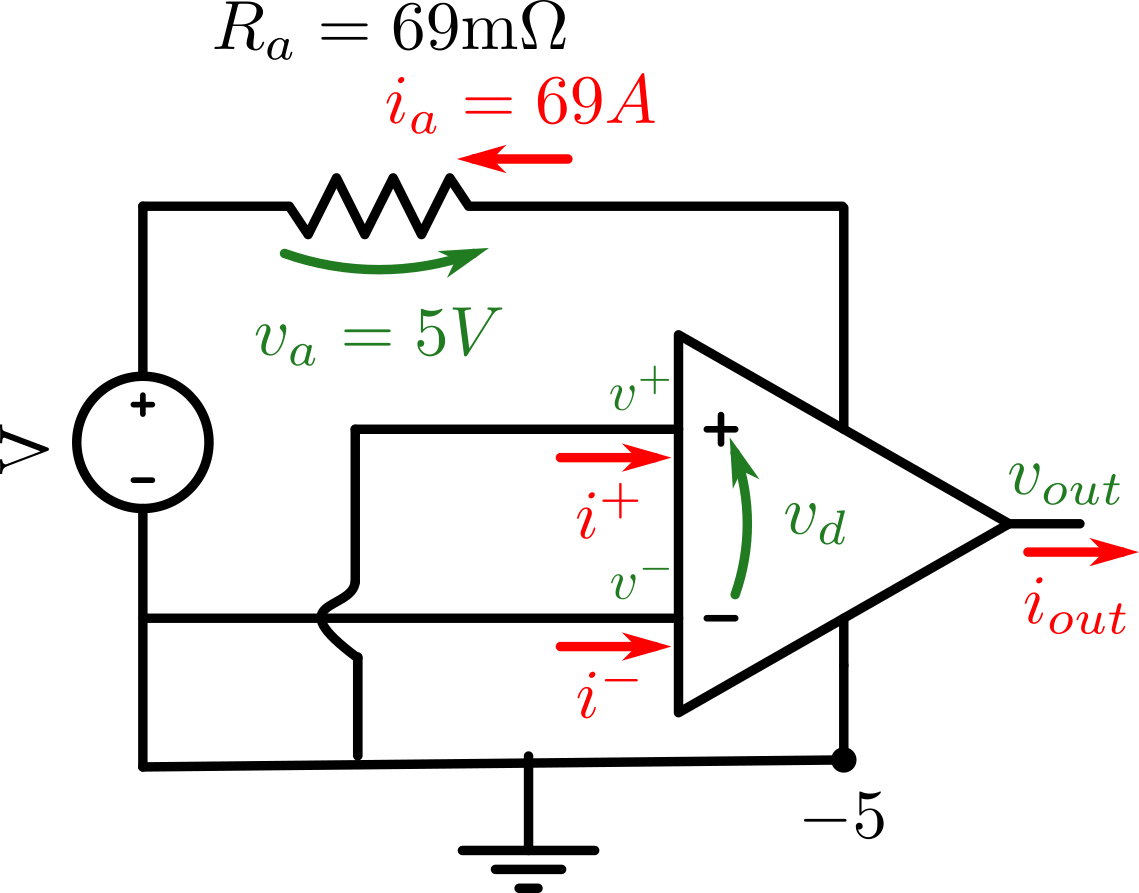
\includegraphics[width=1\linewidth]{Inkscape/electricCircuit.png}
	\caption{Electric Circuit generated using InkScape}
	\label{fig:electriccircuit}
\end{figure}

\chapter{Course Information}
\begin{theorem}{}{}
	Testing my life
\end{theorem}

\begin{definition}{}{}
	Another test
\end{definition}

\begin{example}{}{}
	example
\end{example}

\begin{corollary}{}{}
	More testing
\end{corollary}

\begin{remark}
	Hopefully this course will not be too hard
\end{remark}

\begin{proof}
$$Good at math.$$
\end{proof}
\section{Expectations}
\textbf{Course Objectives}

To introduce students to more advanced concepts pertaining to network
analysis in the time and frequency domain, including the treatment of
active circuits.

\textbf{Learning Outcomes}

At the end of the course, students will be able to \ldots{}

\begin{itemize}
\item
  demonstrate functionality of circuits containing operational
  amplifiers
\item
  assess the performance of circuits that have time dependent responses
\item
  use Laplace transforms to find the response of linear circuits to time
  varying inputs
\item
  solve for zero input and forced response as a function of time using
  node or mesh analysis
\item
  design circuits which have specified transfer functions and meet other
  specified constraints
\item
  evaluate the frequency response of linear circuits and make straight
  line Bode gain and phase plots
\item
  design a cascade of active or passive filter circuits to achieve a
  desired transfer function
\item
  analyze circuits containing coupled inductors and ideal transformers
\item
  evaluate sinusoidal steady state response of linear circuits using
  phasors
\item
  evaluate two port parameters of linear circuits and find the response
  of two ports to external input
\end{itemize}

\textbf{Syllabus}

\begin{quote}
Appr. No of Classes

Introduction
\ldots{}\ldots{}\ldots{}\ldots{}\ldots{}\ldots{}\ldots{}\ldots{}.\ldots{}\ldots{}\ldots{}\ldots{}\ldots{}\ldots{}\ldots{}\ldots{}\ldots{}\ldots{}\ldots{}\ldots{}\ldots{}\ldots{}\ldots{}\ldots{}\ldots{}\ldots{}\ldots{}\ldots{}\ldots{}\ldots{}\ldots{}\ldots{}\ldots{}\ldots{}.
1

Basic Circuit Laws (review)
\ldots{}\ldots{}\ldots{}\ldots{}\ldots{}\ldots{}\ldots{}\ldots{}\ldots{}\ldots{}\ldots{}\ldots{}\ldots{}\ldots{}\ldots{}\ldots{}\ldots{}\ldots{}\ldots{}\ldots{}\ldots{}\ldots{}\ldots{}\ldots{}\ldots{}\ldots{}.
2

Operational Amplifiers
\ldots{}\ldots{}\ldots{}\ldots{}\ldots{}\ldots{}\ldots{}\ldots{}\ldots{}\ldots{}\ldots{}\ldots{}\ldots{}\ldots{}\ldots{}\ldots{}\ldots{}\ldots{}\ldots{}\ldots{}\ldots{}\ldots{}\ldots{}\ldots{}\ldots{}\ldots{}\ldots{}\ldots{}\ldots{}2

Transfer Functions
\ldots{}\ldots{}\ldots{}\ldots{}\ldots{}\ldots{}\ldots{}\ldots{}\ldots{}\ldots{}\ldots{}\ldots{}\ldots{}\ldots{}\ldots{}\ldots{}\ldots{}\ldots{}\ldots{}\ldots{}\ldots{}\ldots{}\ldots{}\ldots{}\ldots{}\ldots{}\ldots{}\ldots{}\ldots{}\ldots{}\ldots{}.
1

Bode Plots
\ldots{}\ldots{}\ldots{}\ldots{}\ldots{}\ldots{}\ldots{}\ldots{}\ldots{}\ldots{}\ldots{}\ldots{}\ldots{}\ldots{}\ldots{}\ldots{}\ldots{}\ldots{}\ldots{}\ldots{}\ldots{}\ldots{}\ldots{}\ldots{}\ldots{}\ldots{}\ldots{}\ldots{}\ldots{}\ldots{}\ldots{}\ldots{}\ldots{}\ldots{}\ldots{}\ldots{}
4

Serial and Parallel Resonance
\ldots{}\ldots{}\ldots{}\ldots{}\ldots{}\ldots{}\ldots{}\ldots{}\ldots{}\ldots{}\ldots{}\ldots{}\ldots{}\ldots{}\ldots{}\ldots{}\ldots{}\ldots{}\ldots{}\ldots{}\ldots{}\ldots{}\ldots{}\ldots{}\ldots{}
1

Filters
\ldots{}\ldots{}\ldots{}\ldots{}\ldots{}\ldots{}\ldots{}\ldots{}\ldots{}\ldots{}\ldots{}\ldots{}\ldots{}\ldots{}\ldots{}\ldots{}\ldots{}\ldots{}\ldots{}\ldots{}\ldots{}\ldots{}\ldots{}\ldots{}\ldots{}\ldots{}\ldots{}\ldots{}\ldots{}\ldots{}\ldots{}\ldots{}\ldots{}\ldots{}\ldots{}\ldots{}\ldots{}\ldots{}.
2

Coupled inductors and transformers
\ldots{}\ldots{}\ldots{}\ldots{}\ldots{}\ldots{}\ldots{}\ldots{}\ldots{}\ldots{}\ldots{}\ldots{}\ldots{}\ldots{}\ldots{}\ldots{}\ldots{}\ldots{}\ldots{}\ldots{}..
1

Laplace Transforms for Circuits
\ldots{}\ldots{}\ldots{}\ldots{}\ldots{}\ldots{}\ldots{}\ldots{}\ldots{}\ldots{}\ldots{}\ldots{}\ldots{}\ldots{}\ldots{}\ldots{}\ldots{}\ldots{}\ldots{}\ldots{}\ldots{}\ldots{}\ldots{}\ldots{}
4

Two-Port Networks
\ldots{}\ldots{}\ldots{}\ldots{}\ldots{}\ldots{}\ldots{}\ldots{}\ldots{}\ldots{}\ldots{}\ldots{}\ldots{}\ldots{}\ldots{}\ldots{}\ldots{}\ldots{}\ldots{}\ldots{}\ldots{}\ldots{}\ldots{}\ldots{}\ldots{}\ldots{}\ldots{}\ldots{}\ldots{}\ldots{}..
4
\end{quote}

\begin{longtable}[]{@{}ll@{}}
\toprule
Sub Total & 22\tabularnewline
Midterm Test & 1\tabularnewline
Review & 1\tabularnewline
Total & 24\tabularnewline
\bottomrule
\end{longtable}

Some of the textbooks used in this course include:
\begin{itemize}
	\item[---]  \hyperlink{ref-book:nilEC}{Nilsson}
	\item[---]  \hyperlink{ref-book:nilECSol}{Nilsson ISM}
	\item[---]  \hyperlink{ref-book:alexEC}{Alexander} 
	\item[---]  \hyperlink{ref-book:alexECSol}{Alexander ISM}
\end{itemize}

\chapter{Concepts to Review}
\section{Components in series and parallel}

Series resistances add:

\[ R_s = R_1 + R_2 + R_3 + \cdots \]

Parallel resistances diminish:

\[ R_p = \frac{1}{ \frac{1}{R_1} + \frac{1}{R_2} + \frac{1}{R_3} + \cdots} \]

Impedances behave like resistances.\\

Series capacitances diminish:

\[ C_s = \frac{1}{ \frac{1}{C_1} + \frac{1}{C_2} + \frac{1}{C_3} + \cdots} \]

Parallel capacitances add:

\[ C_p = C_1 + C_2 + C_3 + \cdots \]

Series inductances add:

\[ L_s = L_1 + L_2 + L_3 + \cdots \]

Parallel inductances diminish:

\[ L_p = \frac{1}{ \frac{1}{L_1} + \frac{1}{L_2} + \frac{1}{L_3} + \cdots} \]

For the special case of two components of the diminshing type (x being a dummy variable):

\[ \frac{1}{ \frac{1}{x_1} + \frac{1}{x_2} } = \frac{x_1 \cdot x_2}{x_1 + x_2} \]

\section{State devices / energy storage devices}
This section assumes time-invariant devices, i.e. capacitance/inductance is a fixed value, and not a function of time.

\subsection{Capacitors}

The current through a capacitor is a function of the \emph{rate of change} of voltage:

\[ i(t) = C \frac{dv(t)}{dt} \]

To find the voltage over a capacitor, we need to know its full history:

\[ v(t) = \frac{1}{C} \int_{-\infty}^{t} i(t) dt \]

... or we can simply do it by knowing the current through it between $t_1$ and $t_2$, plus the initial voltage:

\[ v(t_2) = \frac{1}{C} \int_{t_1}^{t_2} i(t) dt + v(t_1) \]

The energy stored in a capacitor is:

\[ E = \frac{1}{2} C v^2 \]

\subsection{Inductors}

The voltage over an inductor is a function of the \emph{rate of change} of current:

\[ v(t) = L \frac{di(t)}{dt} \]

To find the current through an inductor, we need to know its full history:

\[ i(t) = \frac{1}{L} \int_{-\infty}^t v(t) dt \]

... or we can simply do it by knowing the voltage over it between $t_1$ and $t_2$, plus the initial current through it:

\[ i(t_2) = \frac{1}{L} \int_{t_1}^{t_2} v(t) dt + i(t_1) \]

The energy stored in an inductor is:

\[ E = \frac{1}{2} L i^2 \]

\section{First order circuits}

General equation for an increasing/decaying exponential in a RC/RL circuit:

\[ v = V_S + (V_0 - V_S) e^{-t/RC} \]
\[ i = \frac{V_S}{R} + (i_0 - \frac{V_S}{R}) e^{-Rt/L} \]

where v = the voltage across the capacitor. For RL circuits, replace $V_S$ by the maximum current and $V_0$ by the initial current through the inductor. Above is for a thevenin equivalent circuit.\\

ZIR / Zero Input Response, same as above with $V_S = 0$:

\[ V_0 e^{-t/RC} \]

ZSR / Zero State Response, same as above with $V_0 = 0$:

\[ V_S(1 - e^{-t/RC}) \]

\newpage

\section{Second order circuits, impedance, filters}

Canonical form of the characteristic equation for second-order circuits; use this to match up the values of $\alpha$ and $\omega_0$ for a circuit:

\[ s^2 + 2\alpha s + {\omega_0}^2 = 0 \]

\subsection{For all LC and RLC circuits:}

\[ \text{Natural/undamped resonant radian frequency: } \omega_0 \text{ (rad/s)} \]
\[ \text{Damping factor: } \alpha \text{ (rad/s)} \]

Note that zeta ($\zeta$) is used as a damping factor in many texts; it is defined as
\[ \zeta = \frac{\alpha}{\omega_0} \text{ (dimensionless)} \]

The bandwidth $\Delta \omega$, i.e. the \emph{width} of the frequency \emph{band} that is above $\displaystyle \frac{1}{\sqrt{2}}$ times the input amplitude, is given by

\[ \Delta \omega = 2 \alpha \text{ (rad/s) (measured at } \frac{1}{\sqrt{2}} \text{ points)} \]

\[ \text{Quality factor: } Q = \frac{\omega_0}{2\alpha} \text{ (dimensionless)} \]

RLC circuits can be underdamped, overdamped, or critically damped.

\[ \text{Underdamped: } \omega_0 > \alpha \text{ or, equivalently, } Q > \frac{1}{2} \text { or, equivalently, } \zeta < 1 \]
\[ \text{Overdamped: } \omega_0 < \alpha \text{ or, equivalently, } Q < \frac{1}{2} \text { or, equivalently, } \zeta > 1 \]
\[ \text{Critically damped: } \omega_0 = \alpha \text{ or, equivalently, } Q = \frac{1}{2} \text { or, equivalently, } \zeta = 1 \]

When they are \emph{underdamped}, the \emph{damped resonant frequency} $\omega_d$ is given by
\[ \omega_d = \sqrt{{\omega_0}^2 - \alpha^2} \]
The naming here might be confusing; the \emph{damped} frequency is used for \emph{underdamped} systems. The reason is that the \emph{undamped} frequency is used for systems with no damping whatsoever, i.e. LC circuits with no resistor.\\
Underdamped RLC circuits are the only kind that oscillate, so the natural frequency is less interesting for overdamped circuits.

\subsection{Series RLC circuits}

\[ \omega_0 = \frac{1}{\sqrt{LC}} \text{ rad/s} \]
\[ f_0 = \frac{1}{2\pi \sqrt{LC}} \text { Hz} \]
\[ \alpha = \frac{R}{2L} \text{ rad/s} \]
\[ \Delta \omega = 2\alpha = \frac{R}{L} \text { rad/s} \]
\[ \text{Period: } \frac{2\pi}{\omega_0} = 2\pi \sqrt{LC} \text { seconds} \]
\[ Q = \frac{\omega_0}{2\alpha} = \frac{L}{R\sqrt{LC}} \text { (dimensionless)} \]

\subsection{Parallel RLC circuits}

\[ \omega_0 = \frac{1}{\sqrt{LC}} \text{ rad/s} \]
\[ f_0 = \frac{1}{2\pi \sqrt{LC}} \text { Hz} \]
\[ \alpha = \frac{1}{2RC} \text{ rad/s} \]
\[ \Delta \omega = 2\alpha = \frac{1}{RC} \text { rad/s} \]
\[ \text{Period: } \frac{2\pi}{\omega_0} = 2\pi \sqrt{LC} \text { seconds} \]
\[ Q = \frac{\omega_0}{2\alpha} = \frac{RC}{\sqrt{LC}} \text { (dimensionless)} \]

\subsection{Frequency- to time-domain conversion}
You can find the time-domain behavior of a circuit to sinusoidal input from nothing but a complex amplitude of the form $V_x$:
\[ v_X(t) = |V_x| \cos{(\omega t + \angle V_x)} \]
See below for information about how to calculate the magnitude $|z|$ and the angle $\angle z$ of a complex number.

\subsection{Complex algebra}
A few properties of complex numbers that are necessary to know:

\[ |a + jb| = \sqrt{a^2 + b^2} \]
\[ \angle (a + jb) = \arctan{(\frac{b}{a})} \text{ or, preferably, } \text{atan2}(a, b) \]

\[ |a + j0| = a \text { if $a > 0$; otherwise, the magnitude is just the absolute value } |a| \]
\[ |0 + jb| = b \]
\[ |0 - jb| = b \]

\[ \angle (a + j0) = 0 \]
\[ \angle (0 + jb) = \frac{\pi}{2} \]
\[ \angle (0 - jb) = -\frac{\pi}{2} \]

\[ |z_1 \cdot z_2| = |z_1| \cdot |z_2| \]
\[ \left| \frac{z_1}{z_2} \right| = \frac{|z_1|}{|z_2|} \]

\[ \angle (z_1 \cdot z_2) = \angle z_1 + \angle z_2 \]
\[ \angle \left( \frac{z_1}{z_2} \right) = \angle z_1 - \angle z_2 \]

\subsection{Impedances}

\[ \text{Resistor: } Z_R = R \]
\[ \text{Capacitor: } Z_C = \frac{1}{j\omega C} \]
\[ \text{Inductor: } Z_L = j\omega L \]

%%%%%%%%%%%%%%%%%%%%%%%%
%%% Circuit analysis %%%
%%%%%%%%%%%%%%%%%%%%%%%%

\chapter{Circuit analysis}

\section{Thevenin equivalent circuits}

Say we have an capacitor circuit to analyze:

\begin{figure} \begin{lateximage} \begin{circuitikz}[scale=1.2]
	\draw (0,0) node [ground] {} to [V=$V_S$] (0,3)
	to [R=$R_1$]  (3,3)
	to [R=$R_2$]  (6,3)
	to [C=$C$, v=$v_C$]   (6,0);
	
	\draw (3,3)                  to [R=$R_3$]  (3,0);
	\draw (0,0)                  to           (6,0);
\end{circuitikz} \end{lateximage} \caption{Capacitor Circuit} \end{figure}

Since this is a linear network, we can simplify it by calculating its \emph{Thevenin equivalent}. Consider the network as seen from the port where the capacitor is attached:

\begin{figure} \begin{lateximage} \begin{circuitikz}[scale=1.2]
	\draw (0,0) node [ground] {} to [V=$V_S$] (0,3)
	to [R=$R_1$]  (3,3)
	to [R=$R_2$, -o]  (6,3);
	
	\draw (3,3)                  to [R=$R_3$]  (3,0);
	\draw (0,0)                  to [short, -o]         (6,0);
	\draw (6,0)                  to [open, v>=$V_{TH}$] (6,3);
\end{circuitikz} \end{lateximage} \caption{Thevenin Equivalent} \end{figure}

$V_{TH}$, the open circuit voltage, will be given by the voltage divider formed by $R_3$ and $R_1$:

\[ V_{TH} = \frac{R_3}{R_1 + R_3} \cdot V_S \]

Since no current flows at the port (for the \emph{open circuit} voltage!), $R_2$ doesn't contribute at all.

We also want to measure the resistance ``looking in'' to this port; this will be the Thevenin resistance $R_{TH}$. To do this, we turn off all \emph{independant} voltage and current sources, by replacing all current sources with \emph{opens} and all voltage sources with \emph{short circuits}.\\
Leave dependant sources in the circuit!

\begin{figure} \begin{lateximage} \begin{circuitikz}[scale=1.2]
	\draw (0,0)                  to [short] (0,3)
	to [R=$R_1$]  (3,3)
	to [R=$R_2$, -o]  (6,3);
	
	\draw (3,3)                  to [R=$R_3$]  (3,0);
	\draw (0,0)                  to [short, -o]         (6,0);
	\draw (6,0)                  to [open] (6,3);
\end{circuitikz} \end{lateximage} \caption{Thevenin Equivalent II} \end{figure}

\[ R_{TH} = R_2 + (R_1 || R_3) = R_2 + \frac{R_1 \cdot R_3}{R_1 + R_3} \]

Now that we know the Thevenin voltage $V_{TH}$ and the Thevenin resistance $R_{TH}$, we can replace the circuit with a voltage source of voltage $V_{TH}$ volts in series with a resistor of value $R_{TH}$ ohm, and place the capacitor back into the circuit:

\begin{figure} \begin{lateximage} \begin{circuitikz}[scale=1.2]
	\draw (0,0) node [ground] {} to [V=$V_{TH}$] (0,3)
	to [R=$R_{TH}$] (3,3)
	to [C=$C$, v=$v_C$]      (3,0);
	\draw (0,0)                  to              (3,0);
\end{circuitikz} \end{lateximage} \caption{Thevenin Equivalent III} \end{figure}

Our previous circuit has now turned into a simple RC circuit, which is easier to analyze. See the chapter on RC circuits.\\

As a side note, another way of measuring the Thevenin resistance is to short circuit the output node, calculate/measure the short-circuit current (with all sources left intact, of course), and calculate $R_{TH}$ as $\frac{V_{TH}}{I_{SC}}$.\\

In summary:

$\bullet$ Calculate/measure the open circuit voltage $V_{TH}$ at the port\\
$\bullet$ Turn off all independent sources (make short circuits of voltage sources, and open circuits of current sources), but leave dependant sources intact\\
$\bullet$ Calculate/measure the resistance $R_{TH}$ at the port terminal pair\\
$\bullet$ Replace the original circuit with a series circuit of a voltage source (voltage $V_{TH}$ volts), a resistor (resistance $R_{TH}$ ohm) and the element you want to analyze.

\newpage

\section{Norton equivalent circuits}
Nortan equivalent circuits are very similar to Thevenin equivalents, but use a \emph{current source} in \emph{parallel} with a resistor rather than a \emph{voltage source} in \emph{series} with a resistor.

To convert a circuit to its Norton equivalent:

$\bullet$ Calcurate/measure the \emph{short circuit current}, i.e. the current that would flow through the output port if we were to short-circuit it. The result is the Norton current $I_N$.\\
$\bullet$ Turn off all independent sources (make short circuits of voltage sources, and open circuits of current sources), but leave dependant sources intact.\\
$\bullet$ Calculate/measure the resistance at the port terminal pair; the result is the Norton resistance $R_N$.\\
$\bullet$ Replace the original circuit with a parallel circuit of a current source (current $I_N$ amperes), a resistor (resistance $R_N$ ohm) and the element you want to analyze.\\

\begin{figure} \begin{lateximage} \begin{circuitikz}[scale=1.2]
	\draw (0,0) node [ground] {} to [I=$I_N$] (0,3);
	\draw (0,3) to (3,3);
	\draw (3,3) to [R=$R_N$] (3,0);
	\draw (6,3) to [C=$C$, v=$v_C$] (6,0);
	\draw (6,0) to (0,0);
	\draw (6,3) to (3,3);
\end{circuitikz} \end{lateximage} \caption{Norton Circuit} \end{figure}

Note that since the method for calculating the equivalent resistance is identical for the Thevenin and Norton methods, $R_N = R_{TH}$.
It is easy to convert between one and the other:

\[ R_N = R_{TH} \]
\[ I_N = \frac{V_{TH}}{R_{TH}} \]
\[ V_{TH} = I_N \cdot R_N \]
%\chapter{Operation Amplifiers}
%%% Op amps 

\chapter{Operational Amplifiers}
\paragraph{Intro}
\emph{Operational Amplifiers}, or \emph{op amps}, are an amplifier abstraction; that is, we can use it without knowing about its insides.

The schematic symbol looks like this:\\

\begin{figure} \begin{lateximage} \begin{circuitikz} 
	\draw	(0,0) node[op amp] (opamp) {}
	(opamp.+) node[left] {$v_+$}
	(opamp.-) node[left] {$v_-$}
	(opamp.out) node[right] {$v_o$}
	(opamp.down) node[ground] {}
	(opamp.up) ++ (0,.5) node[above] {$12$ V};
	\draw (0,0.5) to (0,1);
\end{circuitikz} \end{lateximage} \caption{Basic Op Amp} \end{figure}

Above is a \emph{single-supply} op amp, that can output voltages between 0 and 12 volts, with respect to ground. \emph{Dual-supply} op amps are also common; in that case, you'd replace the ground above with -12 volts, and have the ground (which is then not directly connected to the op amp) where the two rails ``meet'', i.e. output range is from 12 volts above ground all the way down to 12 volts below ground.\\
That way, the op amp can output negative voltages (again with respect to the circuit ground), which is often required when dealing with signals such as audio, which are ground referenced and symmetric around the 0 volt axis.\\

The ideal op amp has infinite input impedance, and zero output impedance. Thus, no current flows into the input terminals; all current from the output terminal comes from the power terminals.

In many cases, we don't really care about showing the supply connection explicitly, and instead use the following symbol:\\

\begin{figure} \begin{lateximage} \begin{circuitikz}
	\draw	(0,0) node[op amp] (opamp) {}
	(opamp.+) node[left] {$v_+$}
	(opamp.-) node[left] {$v_-$}
	(opamp.out) node[right] {$v_o$};
\end{circuitikz} \end{lateximage} \caption{Annotated Op Amp} \end{figure}

This document will use the latter symbol from now on.\\

Op amps use a \emph{differential} input. That is to say, neither of the two input connections is necessarily ground, and the amplifier amplifies the \emph{difference} between the two input ports. That is, ideally,

\[ v_o = A (v_+ - v_-) \]
where $A$ is the amplifier's voltage gain. In the ideal op amp model, $A \to \infty$. In real op amps, A is often on the order of 100,000 or more. Needless to say, most of the time, we don't want to amplify a signal that much - even a input voltage difference as tiny as $12 \mu$V would be enough to drive the output to the maximum 12 V ($12 \mu V \cdot 10^6 = 12 V$) for an amplifier with $A = 10^6$, which most certainly exist on the market.\\

So, to summarize what we've seen so far:
\begin{enumerate}
	\item The op amp is a \emph{differential} amplifier ...
	\item ... that outputs a ground-referenced voltage.
	\item Its gain is extremely high (ideally infinite), often on the order of $10000$ to a million, or even higher. If we want less gain, we'll have to take care of that outside the abstract ``amplifier box'' that is the op amp.
	\item Op amps can be powered by a single supply (a positive voltage and ground) or a dual supply (a positive and a negative voltage, with ground being in between the two). There are op amps made specifically for either of these two, though many works in either configuration.
\end{enumerate}

To analyze circuits with ideal op amps, we model them as a VCVS, that is, a voltage-controlled voltage source. Again, no current flows into the input terminals, so we model them as open circuits.\\

\begin{figure} \begin{lateximage} \begin{circuitikz}[scale=1.2]
	\draw (1,2.5) node{\hspace{-20px} $v_{+}$} to [short, i={$i_{+} \approx 0$}] (3,2.5);
	\draw (1,1.5) node{\hspace{-20px} $v_{-}$} to [short, i={$i_{-} \approx 0$}] (3,1.5);
	\draw (4,0) to node [ground] {} (4, 1) to [cV] (4,3);
	\draw (4,3) to [short, -o] (6,3);
	\draw (6,1.5) [short, o-] {} to (6,1.25) node [ground] {};
	\draw (5.75,2.75) to [open, v^=$v_o$] (5.75,1.75);
\end{circuitikz} \end{lateximage} \caption{Op Amp with VCVS} \end{figure}

Since real-life op amps are powered by a power supply (rather than being ideal sources themselves), they can never output a voltage that is higher than that of the power supply. Thus, when the difference between the inputs is greater than $\displaystyle \frac{\text{Power supply voltage}}{\text{Gain}}$, the op amp \emph{saturates}, and the output stays close to the power supply rail.\\
Here's a plot of an op amp's transfer function, with a gain of $10^6$:

\begin{comment}
%%% Mathematica source code

% Emulate saturation
f[x_] = If[-12*10^-6 <= x <= 12*10^-6, x * 10^6, Sign[x] * 12]

Plot[f[x], {x, -18 * 10^-6, 18 * 10^-6}, PlotRange -> Full,
Ticks -> {
{
{-12*10^-6, "-12\[Mu]V"}, {-6*10^-6, "-6\[Mu]V"}, {6*10^-6 , 
"6\[Mu]V"}, {12*10^-6, "12\[Mu]V"}
}, 
{
{-12, "-12V"}, {-6, "-6V"}, {6, "6V"}, {12, "12V"}
}
}, GridLines -> {
{12 * 10^-6, -12 * 10^-6}, None
},
GridLinesStyle -> Dotted,
AxesLabel -> {"\!\(\*SubscriptBox[\(v\), \(i\)]\)", 
"\!\(\*SubscriptBox[\(v\), \(o\)]\)"}]
%%% End mathematiac source code
\end{comment}

%\includegraphics[scale=1.5]{Graphics/opamp_transfer_function}

Note the extreme difference in scale between the axes: the $v_i$ axis is in microvolts, while the $v_o$ axis is in volts. The op amp behaves linearly as long as the gain multiplied by the input voltage difference is less than the power supply voltage (we call this the \emph{active region}, or sometimes the linear region), but \emph{saturates} whenever the voltage difference is greater.\\

Most op amps can't bring the output very close to either power supply rail; an op amp powered by a $\pm12$ V supply can usually swing between roughly -11 and +11 volts, or thereabouts. Therefore, an op amp will generally saturate before it the power supply voltage. Op amps which can output very close (usually within a few millivolts) of the power rails are called \emph{rail-to-rail output} op amps. There are also \emph{rail-to-rail input} and \emph{rail-to-rail input/output} (RRIO) op amps.

\paragraph{Noninverting amplifier}
Let's use an op amp to build a noninverting amplifier, one of the simpler (and perhaps more common) uses of an op amp. This configuration uses a resistive divider between the output and the $v_-$ terminal to limit the gain to more usable values. This also has the huge advantage of making the op amp very stable, as opposed to its ``raw'' form, where the gain $A$ can vary extremely much for pretty much no discernable reason.\\
It looks something like this:\\

\begin{figure} \begin{lateximage} \begin{circuitikz}
	\draw (0,3) node[op amp, yscale=-1] (opamp) {} (0, 0);
	
	% Node voltage labels. Ugly hack!
	\draw (opamp.+) to [open] (-1.3, 3.25) node {$v_+$};
	\draw (opamp.-) to [open] (-1.3, 2.7) node {$v_-$};
	
	% v_- label at the divider
	\draw (2,1) to [open] (2.5,1) node {$v_-$};
	
	% Voltage source, output label, v_- to divider
	\draw (opamp.+) to (-3, 3.5) to [sV=$v_I$] (-3, -1) node [ground] {};
	\draw (opamp.out) to [short, -o] (3.5, 3) node {\quad\quad $v_o$};
	\draw (opamp.-) to (-1.6, 2.5) to (-1.6, 1) to (2, 1);
	
	\draw (2, 3) to [R=$R_1$, *-*] (2, 1)
	to [R=$R_2$, *-]  (2, -1);
	\draw (2, -1) node [ground] {} to (2, -1);
\end{circuitikz} \end{lateximage} \caption{Noninverting Op Amp} \end{figure}\ \\

As always, $v_o$ is ground-referenced, though that will not be shown explicitly here or in future circuit diagrams.\\
Let's analyze this circuit. First, we know that the op amp input/output relation is, always,

\[ v_o = A(v_+ - v_-) \]

Let's find the values of $v_+$ and $v_-$ for this circuit.\\
$v_+$ is simply our input voltage $v_I$.\\
$v_-$ is given by a simple voltage divider between $v_o$ and ground, so

\[ v_- = v_o \cdot \frac{R_2}{R_1 + R_2} \]

(Remember that $v_-$ is an open circuit; the input impedance is infinite, and the connection there doesn't affect the voltage divider ratio.)\\

Let's substitute these values back into the first equation, and get:

\[ v_o = A(v_I - v_o \cdot \frac{R_2}{R_1 + R_2}) \]
\[ v_o = Av_I - A v_o \cdot \frac{R_2}{R_1 + R_2} \]

We have $v_o$ terms on both sides; let's collect all $v_o$ terms on the left-hand side:

\[ v_o + A v_o \cdot \frac{R_2}{R_1 + R_2} = A v_I  \]
\[ v_o(1 + A \cdot \frac{R_2}{R_1 + R_2}) = A v_I \]

Now we can simply divide both sides by the expression multiplying $v_o$ and we're pretty much done:

\[ v_o = \frac{A v_I}{1 + A \cdot \frac{R_2}{R_1 + R_2}} \]

Note that if $\displaystyle A \cdot \frac{R_2}{R_1 + R_2} \gg 1$, we can ignore the $1$ term without losing any noteworthy amount of precision. For example, if $A = 10^6$, $R_1 = 3000$ and $R_2 = 1000$, which gives a gain of 3.999984, the value we get using the approximation (ignoring the $1$) is exactly $4$. Such tiny errors don't really matter to us, so we can say that

\[ v_o \approx \frac{A v_I}{A \cdot \frac{R_2}{R_1 + R_2}} \]

Note that we can now cancel out the $A$ terms!

\[ v_o \approx \frac{v_I}{\frac{R_2}{R_1 + R_2}} = v_I \cdot \frac{R_1 + R_2}{R_2} \]

Therefore, this configuration gives a voltage gain of almost exactly $\displaystyle \frac{R_1 + R_2}{R_2} = 1 + \frac{R_1}{R_2}$, as long as we make sure that $\displaystyle A \cdot \frac{R_2}{R_1 + R_2} \gg 1$ is true, by making sure we never make $R_1$ much, much bigger than $R_2$. However, even when $R_1$ is \emph{1000 times} greater than $R_2$, the approximation works out quite well: for $A = 10^6$, $R_1 = 10^6$ $\Omega$ and $R_2 = 1000$ $\Omega$ the error is about 0.1\%. Such a configuration would give a gain of roughly 1000.\\

So, this circuit works! It gives as a gain we can set via simple resistor values, and thus the op amp gain $A$ is virtually irrelevant to this circuit, as long as it's very large.\\
The question is, though, \emph{how} does it work? The answer is that the resistor divider connected to the inverting input creates a \emph{negative feedback} loop.

\newpage

\paragraph{Negative feedback}
Negative feedback is a quite simple concept. This explanation may be a bit confusing at first, but think it through carefully and you should get it - and when you do, you'll agree that it's simple! I'll copy the schematic from above for convenience:\\

\begin{figure} \begin{lateximage} \begin{circuitikz}
	\draw (0,3) node[op amp, yscale=-1] (opamp) {} (0, 0);
	
	% Node voltage labels. Ugly hack!
	\draw (opamp.+) to [open] (-1.3, 3.25) node {$v_+$};
	\draw (opamp.-) to [open] (-1.3, 2.7) node {$v_-$};
	
	% v_- label at the divider
	\draw (2,1) to [open] (2.5,1) node {$v_-$};
	
	% Voltage source, output label, v_- to divider
	\draw (opamp.+) to (-3, 3.5) to [sV=$v_I$] (-3, -1) node [ground] {};
	\draw (opamp.out) to [short, -o] (3.5, 3) node {\quad\quad $v_o$};
	\draw (opamp.-) to (-1.6, 2.5) to (-1.6, 1) to (2, 1);
	
	\draw (2, 3) to [R=$R_1$, *-*] (2, 1)
	to [R=$R_2$, *-]  (2, -1);
	\draw (2, -1) node [ground] {} to (2, -1);
\end{circuitikz} \end{lateximage} \caption{Negative feedback Op Amp} \end{figure}

\ \\

Let's think about how this circuit works. Say $v_I$ is a static value of 5 volts, and $R_1 = R_2$ (in which case their actual values won't matter). The node voltage $v_-$ will be exactly half of $v_o$. $v_o$, in turn, will be (according to the gain equation we found) $\displaystyle v_I \cdot \frac{R + R}{R} = 2\cdot v_I$.\\
So, to begin with, we have

\[ v_I = v_+ = 5 V \]
\[ v_o = 2\cdot v_I = 10 V \]
\[ v_- = \frac{v_o}{2} = 5 V \]

... Well, $v_+ \neq v_-$, but they're very, very close to equal. If they were exactly equal, $v_o$ would be the gain times 0 ($A(v_+ - v_-) = 10^6(5 - 5) = 0$), which clearly isn't the case here. The difference depends on the op amp's gain $A$, but will be on the order of microvolts for a gain of $10^6$. For now, we'll consider them equal, to drive home the point of negative feedback. In reality, $v_o$ is just ever so slightly different than $2 \cdot v_I$.\\

So, right now, $v_+ = v_- = 5 V$, and $v_o = 10 V$. Now, let's think about what would happen if, for whatever reason (op amp instability, external noise, etc.) the voltage at node $v_o$ suddenly increased to, say, 12 volts, without a change in the input.\\
Clearly, the voltage $v_+$ would remain unchanged; it will always stay at 5 volts due to the voltage source being directly connected there.\\
$v_-$, on the other hand, is half of $v_o$, and so that node would become $6$ volts.\\
So now, after this output voltage bump, we have $v_+ = 5$, $v_- = 6$ and $v_o = 12$. What happens then?\\

Well, again, we have the op amp equation: $v_o = A(v_+ - v_-) = A(5 - 6) = -A$. In words, the op amp would try, as best it could, to drive the voltage $v_o$ down to $-10^6$ volts (using the gain $A=10^6$ we've been using so far). Needless to say it couldn't, due to the limited power supply, but it would try really hard to bring the voltage at the output node down.\\
Let's say it managed to drive the output down to 8 volts in a short time period. At that point, $v_+ = 5V$, $\displaystyle v_- = \frac{8}{2} = 4V$, which means the op amp would try to drive the output \emph{up} really hard, since $v_+ > v_-$, and so on.\\
In practice, the output wouldn't fluctuate this much; rather, the reaction would be fast enough that the change virtually doesn't happen in the first place. This \emph{can} certainly lead to unwanted oscillations, but that topic is a bit too advanced for this section and chapter.\\

The important point here is that the negative feedback loop causes the op amp to do whatever it can on the output to keep the two inputs very close to each other. If the output rises too high, causing $v_-$ to increase above $v_+$, it tries to reduce the output voltage to compensate. If the output drops too low, causing $v_-$ to drop below $v_+$, it tries to increase the output voltage to compensate.\\
This is a \emph{negative feedback loop}, a concept which can be applied to many situations, including many not in electronics.

In negative feedback, a gap between the output and expected output will be used to \emph{reduce} this gap, and bring the output closer to the expected value. Therefore negative feedback helps the system become stable.\\

Positive feedback is, as one might expect, the opposite. With positive feedback, a small gap between the expected and actual values will be used to create an even bigger gap, which in turn will increase the amount of feedback, and make the gap larger yet, etc. A common example is when a microphone picks up sound from a nearby speaker, causing the sound from the microphone to be sent to the speaker, which leads to more sound being picked up by the microphone, increasing the volume in a loop until only an extremely loud noise remains.

\paragraph{Virtual short/virtual ground}

When we have an op amp with negative feedback (and \emph{only} when we have negative feedback!), the feedback causes $v_-$ to be almost equal to $v_+$. We can show this by rearranging the gain equation:

\[ v_o = A(v_+ - v_-) \]
\[ v_+ - v_- = \frac{v_o}{A} \]

If we have a typical op amp with a very high gain, let's continue assuming $10^6$, this means that for $v_o$ in the typical range of $\pm 20V$ or less, the difference between $v_+$ and $v_-$ will never be larger than on the order of $\displaystyle \frac{20V}{10^6} = 20 \mu V$.\\
Since a short circuit means a zero (or, with wires that have resistances, just a very small) voltage difference, this is referred to as a \emph{virtual short}, or (especially when $v_+$ is tied to ground) as a \emph{virtual ground}.

This leads to us having three useful constraints when dealing with op amp circuits with negative feedback:

\[ i_+ \approx 0 \]
\[ i_- \approx 0 \]
\[ v_+ \approx v_- \]

When combined, these constraints give rise to a new, very easy method of analysis for these circuits, as we'll see in the following sections.

\newpage

\paragraph{Op amps as buffers}

Let's see what happens if we take the noninverting amplifier in the section above, and instead of coupling $v_o$ to $v_-$ through a voltage divider, we simply connect them with a wire.\\
Since this connection provides negative feedback, we can analyze it extremely easily using the virtual short method outlined above.\\

\begin{figure} \begin{lateximage} \begin{circuitikz}
	\draw (0,3) node[op amp, yscale=-1] (opamp) {} (0, 0);
	
	% Node voltage labels. Ugly hack!
	\draw (opamp.+) to [open] (-1.3, 3.25) node {$v_+$};
	\draw (opamp.-) to [open] (-1.3, 2.7) node {$v_-$};
	
	% v_- label at the divider
	\draw (2,1) to [open] (2.5,1) node {$v_-$};
	
	% Voltage source, output label, v_- to divider
	\draw (opamp.+) to (-3, 3.5) to [sV=$v_I$] (-3, -1) node [ground] {};
	\draw (opamp.out) to [short, -o] (3.5, 3) node {\quad\quad $v_o$};
	\draw (opamp.-) to (-1.6, 2.5) to (-1.6, 1) to (2, 1) to [short, -*] (2,3);
	
\end{circuitikz} \end{lateximage} \caption{Op Amps Voltage Divider} \end{figure}
\ \\

First, we note that $v_+ = v_I$. Via the virtual short, this means that $v_- \approx v_I$. Since $v_o = v_-$ via the wire they share, we draw the conclusion that $v_o \approx v_I$. Well, that was quick!\\

This circuit is known as a buffer, or source follower. It presents a very large (ideally infinite) impedance towards the input $v_I$, so that only a very small current is drawn. However, the op amp's output can deliver an ideally infinite current (which is very far from true in practice, as signal op amps, as opposed to power op amps, are often limited to less than 50 or so milliamps).\\
However, even if the op amp were to be limited to a 10 mA output current, the buffer could still be useful, as many voltage sources such as sensitive sensors may be unable to provide even 1 mA without negative effects. Thus, even a trivial task such as connecting the sensor to some reader, perhaps an ADC (analog-to-digital converter) in a microcontroller, may not work without buffering the voltage first.\\

We can also build inverting buffers; see the next section.

\newpage

\paragraph{Inverting amplifier}

Another amplifier topology that uses negative feedback is the \emph{inverting} amplifier, which causes e.g. a 1 volt signal to become $-1 \cdot G$ at the output, where $G$ is the circuit's gain, set by $R_1$ and $R_2$.

\begin{figure} \begin{lateximage} \begin{circuitikz}
	\draw	(5,2) node[op amp] (opamp) {}  (0,2.5) 
	to [R=$R_2$, i>=$i$] (opamp.-)  (0,2.5);
	\draw (0,0.5) node [ground] {} to [V=$v_I$] (0,2.5);
	
	\draw (3.8,0.5) node [ground] {} to (opamp.+);
	
	\draw (opamp.-) to [open] (3.35, 3.5) node {$v_-$};
	
	\draw (3.8,3.5) to 
	[R=$R_1$, v=$v_{R1}$, i>=$i$] (6.2,3.5)  (3.8,3.5) to 
	[short, -*] (opamp.-)  (6.2,3.5) to 
	[short, -*] (opamp.out)  (opamp.out) to 
	[short, -o] (7, 2) to (7,2) node {\quad\quad $v_o$};  
	
\end{circuitikz} \end{lateximage} \caption{Inverting amplifier} \end{figure}

\ \\
Since this circuit also uses negative feedback, we can use the virtual short method to analyze it quickly.\\
First, we note that $v_+$ is tied to ground, i.e. 0 volts. Therefore, by the virtual short constraint, $v_-$ will be approximately 0 volts. Since by our definitions no current flows into the inverting input ($i_- = 0$), and we take $v_- = 0$, the current $i$ through $R_2$ must be simply $\displaystyle \frac{v_I - 0}{R_2}$. Since, again, no current flows into the inverting input, the same current $i$ must flow through $R_1$ as they are then in series.\\ Therefore, the voltage drop across $R_1$ is that current times the resistance, or

\[ v_{R1} = \frac{v_I}{R_2} \cdot R_1 \] 

The current flows left to right (because of $v_I$ being the driver towards the inverting input at 0 volts), which means the \emph{positive} side of the drop is to the left of $R_1$ (see the above circuit). Therefore, the node $v_o$ is equal to the voltage at $v_-$ minus that resistor drop:

\[ v_o = 0 - \frac{v_I}{R_2} \cdot R_1 = -v_I \cdot \frac{R_1}{R_2} \]

That concludes our analysis! The circuit is indeed inverting, and the (negative) gain is simply $\displaystyle \frac{R_1}{R_2}$.

For the record, the full expression that governs the behavior of this circuit, without the simplifications, is

\[ v_o = -\frac{A v_I R_1}{R_1 + R_2 + A R_2} \]

... from an analysis that was performed, but was not outlined in these notes.\\
As $A \to \infty$, the $R_1 + R_2$ term in the denominator becomes irrelevant, and expression reduces down to one where we can cancel out the As:

\[ v_o \approx -\frac{\cancel{A} v_I R_1}{\cancel{A} R_2} = -v_I \cdot \frac{R_1}{R_2} \]

\ \\
Note that if $R_1 = R_2$, this circuit simply inverts the input, and is therefore an \emph{inverting buffer}, or \emph{unity gain inverting amplifier}, which can certainly be useful.\\

The input impedance of this circuit, that is, $\displaystyle \frac{v_I}{i_I}$, where $i_I$ is the current flowing from the input voltage source, is

\[ R_i = \frac{R_1}{A + 1} + R_2 \]

Thus, as $A \to \infty$ (or just becomes ``very large''), the first term is generally irrelevant, and we can say that $R_i \approx R_2$.

\newpage

\paragraph{Op amp subtractor}
Let's analyze this circuit:

\begin{figure} \begin{lateximage} \begin{circuitikz}
	% Op amp
	\draw	(5,2) node[op amp] (opamp) {}  (0,2.5) 
	to [R, l=$R_1$, i>=$i$] (opamp.-)  (0,2.5);
	% v2 and ground
	\draw (0,0.5) node [ground] {} to [V=$v_2$] (0,2.5);
	
	% v- label		
	\draw (opamp.-) to [open] (3.35, 3.5) node {$v_-$};
	
	% Bottom R2 and ground
	\draw (3.8,-1.5) node [ground] {} to [R=$R_2$] (3.8,1); 
	\draw (3.8, 1) to (opamp.+);
	
	% Bottom R1 and v1
	\draw (1.5,1.5) [R=$R_1$, -*] to (opamp.+);
	\draw (1.5,-1.5) node [ground] {} to [V=$v_1$] (1.5,1) -- (1.5,1.5);
	
	% Upper R2 and connection to output
	\draw (3.8,3.5) to 
	[R, l=$R_2$, v=$v_{R2}$, i>=$i$] (6.2,3.5)  (3.8,3.5) to 
	[short, -*] (opamp.-)  (6.2,3.5) to 
	[short, -*] (opamp.out)  (opamp.out) to 
	[short, -o] (7, 2) to (7,2) node {\quad\quad $v_o$};  
	
\end{circuitikz} \end{lateximage} \caption{Op Amp subtractor} \end{figure}

\ \\
As with the rest of the op amp circuits we've analyzed, this one uses negative feedback (see $R_2$), so we will again use the virtual short method to analyze it. However, this analysis is slightly more complex than the previous ones, due to more algebra at the end.\\
Anyway, let's get started.\\

Since the noninverting ($+$) input doesn't draw any current, the voltage at $v_+$ is given by the voltage divider formed by the $v_1$ - $R_1$ - $R_2$ series circuit:

\[ v_+ = v_1 \cdot \frac{R_2}{R_1 + R_2} \]

By the virtual short method, $v_- = v_+$:

\[ v_- = v_+ \]

Therefore, since we know $v_-$ and $v_2$, we can calculate the current through $R_1$, which we'll simply call $i$:

\[ i = \frac{v_2 - v_-}{R_1} \]

Note that, since the inverting ($-$) input draws no current, all of this current must flow through $R_2$ as well (see the circuit diagram). Therefore, the we can easily calculate the voltage drop across $R_2$ as current times resistance, or

\[ v_{R2} = \frac{v_2 - v_-}{R_1} \cdot R_2 \] 

By know, we know $v_-$, and we know the voltage drop across $R_2$. Since that voltage drop is positive ``towards the left'', $v_o$ will be $v_-$ \emph{minus} the drop across $R_2$:

\[ v_o = v_- - v_{R2} \]
\[ v_o = v_- - \frac{v_2 - v_-}{R_1} \cdot R_2 \]

Let's gather the $v_-$ terms together:

\[ v_o = v_-(1 + \frac{R_2}{R_1}) - \frac{v_2}{R_1} \cdot R_2 \]
\[ v_o = v_-(1 + \frac{R_2}{R_1}) - v_2 \cdot \frac{R_2}{R_1} \]

Let's substitute in $v_-$; remember, it's equal to the expression we have for $v_+$:

\[ v_o = (v_1 \cdot \frac{R_2}{R_1 + R_2}) (1 + \frac{R_2}{R_1}) - v_2 \cdot \frac{R_2}{R_1} \]

What a mess. Let's rewrite $\displaystyle 1 + \frac{R_2}{R_1}$:

\[ v_o = (v_1 \cdot \frac{R_2}{R_1 + R_2}) (\frac{R_1 + R_2}{R_1}) - v_2 \cdot \frac{R_2}{R_1} \]

Aha! Now we can cancel out those $R_1 + R_2$ terms:

\[ v_o = v_1 \cdot \frac{R_2}{R_1} - v_2 \cdot \frac{R_2}{R_1} \]

\[ v_o = \frac{R_2}{R_1} \left(v_1 - v_2 \right) \]

As promised in the section title, this is an op amp \emph{subtractor} circuit. It calculates $v_1 - v_2$, scaled by the ratio of $R_2$ to $R_1$.

\paragraph{Summing amplifier}
Since the previous section covered an op amp subtractor, let's cover an adder, usually called a \emph{summing amplifier}:\\

\begin{figure} \begin{lateximage} \begin{circuitikz}
	% Op amp
	\draw	(5,2) node[op amp] (opamp) {}  (0,2.5);
	
	% RF and connection to output
	\draw (3.8,3.5) to 
	[R=$R_F$] (6.2,3.5) (3.8,3.5) to 
	[short, -*] (opamp.-)  (6.2,3.5) to 
	[short, -*] (opamp.out)  (opamp.out) to 
	[short, -o] (7, 2) to (7,2) node {\quad\quad $v_o$};  
	
	% RS and grounding, v- label
	\draw (1.5,2.5) [R=$R_S$] to (opamp.-);
	\draw (1.5,2.25) node [ground] {} to (1.5,2.5);
	\draw (opamp.-) to [open] (3.35, 3.5) node {$v_-$};
	
	% The long wire to the + input
	\draw (0.5, 1.5) [short, *-] to (opamp.+);
	
	% v2 and RI
	\draw (0.5, 1.5) to [R=$R_I$] (-1.5, 1.5);
	\draw (-1.5, 0) node [ground] {} to [V=$v_2$] (-1.5, 1) -- (-1.5, 1.5);
	
	% v1 and RI
	\draw (0.5, 1.5) to (0.5, 2.75) to [R=$R_I$] (-1.5, 2.75) -- (-3, 2.75);
	\draw (-3, 0) node [ground] {} to [V=$v_1$]  (-3, 1) -- (-3, 2.75);
	
\end{circuitikz} \end{lateximage} \caption{Summing amplifier} \end{figure}

\ \\
Yet again, this circuit uses negative feedback, so we can use the virtual short method.\\
First, we can figure out $v_+$. Since no current passes through the noninverting ($+$) input, we can find $v_+$ by analysing the $v_1$ - $R_I$ - $R_I$ - $v_2$ subcircuit.\\
Since it's linear, we can use superposition, and figure out the voltage due to $v_1$ acting alone ($v_{+1}$) and $v_2$ acting alone ($v_{+2}$). To use superposition, we ``set one source to zero'' at a time, which for voltage sources means shorting it out. For $v_1$:

\[ v_{+1} = v_1 \cdot \frac{R_I}{R_I + R_I} = \frac{v_1}{2} \]
(since the resistors have the same value.)\\

Similarly, for $v_2$:

\[ v_{+2} = v_2 \cdot \frac{R_I}{R_I + R_I} = \frac{v_2}{2} \]

So, the sum of the responses will be $v_+$:

\[ v_+ = \frac{v_1 + v_2}{2} \]

By the way, note that if the resistors had unequal values, the above would change. Not only would they not be divided by exactly two, but we would get a \emph{weighted average}, since the top resistor in this schematic is in the numerator for the $v_2$ divider, while the bottom resistor is in the numerator for $v_1$.\\
If we relabel the top resistor $R_1$ and the bottom resistor $R_2$, and set $R_1 = 1000$, $R_2 = 3000$:

\[ v_+ = v_1 \cdot \frac{R_2}{R_1 + R_2} + v_2 \cdot \frac{R_1}{R_1 + R_2} = \frac{3 v_1}{4} + \frac{v_2}{4} \]

\ \\
After that aside, let's get back on track. We found $v_+$, and via the virtual short method, $v_- = v_+$.\\

There are several ways to find $v_o$ from here, but the node method gives a solution with only minor algebra. We set up a node equation for $v_-$:

\[ \frac{v_-}{R_S} + \frac{v_- - v_o}{R_F} = 0 \]

Move $v_o$ to the right-hand side and multiply both sides by $R_F$:

\[ \frac{R_F v_-}{R_S} + v_- = v_o \]

Switch the sides for clarity and factor out $v_-$:

\[ v_o = \frac{R_F v_-}{R_S} + v_- \]
\[ v_o = v_-(\frac{R_F}{R_S} + 1) \]

And, finally, get the actual value of $v_-$ in there:

\[ v_o = \frac{v_1 + v_2}{2} (\frac{R_F}{R_S} + 1) \]

We're done! We can also easily see that if we set $R_F = R_S$, the output is simply $v_o = v_1 + v_2$.

%\newpage

\paragraph{Op amp integrator}
Due to some magic of capacitors, we can use op amps to create circuits that integrate and differentiate signals (with respect to time). Here's an integrator circuit:

\begin{figure} \begin{lateximage} \begin{circuitikz}
	% Op amp
	\draw	(5,2) node[op amp] (opamp) {}  (0,2.5);
	
	% Feedback/integrator cap, connection to output
	\draw (3.8,3.5) to 
	[C=$C$, v=$v_C$, i>=$i$] (6.2,3.5) (3.8,3.5) to 
	[short, -*] (opamp.-)  (6.2,3.5) to 
	[short, -*] (opamp.out)  (opamp.out) to 
	[short, -o] (7, 2) to (7,2) node {\quad\quad $v_o$};  
	
	% Grounded noninverting input
	\draw (3.8, 1) node [ground] {} to (opamp.+);
	
	% Voltage source, resistor
	\draw (1, 1) node [ground] {} to [V=$v_I$] (1,2.5);
	\draw (1,2.5) to [R=$R$, i>=$i$] (opamp.-);
	
\end{circuitikz} \end{lateximage} \caption{Op amp integrator} \end{figure}

\ \\
How does this circuit work? Well, remember the formula for the voltage over a capacitor:

\[ v_C = \frac{1}{C} \int_{-\infty}^{t} i(t) dt \]

$v_+$ is grounded, and thus at 0 volts. $v_-$ is, via the virtual short technique, also 0 volts. Therefore, the current through $R$ is simply $\displaystyle \frac{v_I}{R}$.\\
That same current must go through the capacitor, since there's no other way (the noninverting input has an infinite impedance), so the capacitor voltage drop is

\[ v_C = \frac{1}{C} \int_{-\infty}^{t} \frac{v_I}{R} dt = \frac{1}{RC} \int_{-\infty}^{t} v_I dt \]

As with the previous op amp circuits where the noninverting input is grounded, we can find $v_o$ as

\[ v_o = v_- - v_C = 0 - \frac{1}{RC} \int_{-\infty}^{t} v_I dt \]

\[ v_o = -\frac{1}{RC} \int_{-\infty}^{t} v_I dt \]

Thus this is an inverting integrator. If needed, we could feed the output into an inverting buffer (aka inverting unity-gain amplifier) to get it positive.\\

If we do a more complete analysis, we get the differential equation
\[ RC(1 + A) \frac{dv_-}{dt} + v_- = v_I \]
indicating that the time constant for this circuit is multiplied by the op amp gain $A$. Therefore, the equation that describes $v_o$ for a step input is of the same form as we've seen in regular series RC circuits:
\large
\[ v_o = -AV(1 - e^{-\frac{t}{(1 + A)RC}}) \]
\normalsize
... where V is the voltage of the step input.\\
Thus, for short time scales (short compared to $(1 + A)RC$), this circuit is a very good approximation of an ideal integrator.

\paragraph{Op amp differentiator}

\begin{figure} \begin{lateximage} \begin{circuitikz}
	% Op amp
	\draw	(5,2) node[op amp] (opamp) {}  (0,2.5);
	
	% Feedback resistor, connection to output
	\draw (3.8,3.5) to 
	[R=$R$, v=$v_R$, i>=$i$] (6.2,3.5) (3.8,3.5) to 
	[short, -*] (opamp.-)  (6.2,3.5) to 
	[short, -*] (opamp.out)  (opamp.out) to 
	[short, -o] (7, 2) to (7,2) node {\quad\quad $v_o$};  
	
	% Grounded noninverting input
	\draw (3.8, 1) node [ground] {} to (opamp.+);
	
	% Voltage source, capacitor
	\draw (1, 1) node [ground] {} to [V=$v_I$] (1,2.5);
	\draw (1,2.5) to [C=$C$, i>=$i$] (opamp.-);
	
\end{circuitikz} \end{lateximage} \caption{Op amp differentiator} \end{figure}

\ \\
This circuit is identical to the integrator except for \emph{one} change: the capacitor and resistor places have been swapped. So, how does this work, then?\\

$v_+$ is grounded, and so via the virtual short method, $v_-$ must also be 0 volts. Therefore, the voltage drop across the capacitor equals $v_I$. The current through the capacitor is given by

\[ i = C \frac{dv_I}{dt} \]

That same current $i$ is then forced through the resistor $R$, which causes a voltage drop of $R \cdot i$ across the resistor:

\[ v_R = RC \frac{dv_I}{dt} \]

And, as with several of the previous circuits, $v_o$ equals $v_-$ minus the drop across the resistor:

\[ v_o = v_- - v_R = 0 - RC \frac{dv_I}{dt} \]
\[ v_o = - RC \frac{dv_I}{dt} \]

So, as with the previous circuit, this one also inverts. And, again, we could pass it through an inverting buffer op amp to get rid of the inversion.

\paragraph{Buffered filters}
Consider a basic passive RC filter:\\

\begin{figure} \begin{lateximage} \begin{circuitikz}
	
	\draw (3, 0) [R=$R$] to (5, 0) to [C=$C$] (5,-2);
	\draw (2,-2) -- (7,-2); % bottom rail
	\draw (2,0) to (3,0); % top left to R
	\draw (5, 0) to (7,0); % top right, from R
	
	% Voltage labels
	\draw (2,0) to [open, v=$V_i$, o-o] (2, -2);
	\draw (7,0) to [open, v=$V_o$, o-o] (7, -2);
	
	% Filter box
	\draw [dashed] (3,0.8) -- (6, 0.8) -- (6, -2.5) -- (3, -2.5) -- (3, 0.8);
	
\end{circuitikz} \end{lateximage} \caption{Buffered filters} \end{figure}

\ \\
The dashed lines represent the filter components (the reason for them will be clear soon).\\
We've analyzed this circuit in a previous chapter. However, let's look at how a more complete circuit might look, when we attach a Thevenin equivalent source and a resistive load (perhaps a speaker):\\

\begin{figure} \begin{lateximage} \begin{circuitikz}
	
	\draw (3, 0) [R=$R$] to (5, 0) to [C=$C$] (5,-2);
	\draw (0.5,-2) -- (7.5,-2); % bottom rail
	%\draw (2,0) to (2.75,0); % top left to R
	\draw (0.5, 0) to (0.75, 0); % source to RTH
	\draw (2.75, 0) to (3, 0); % RTH to R
	\draw (5, 0) to (7.5,0); % top right, from R
	
	% Voltage labels
	%\draw (2,0) to [open, v=$V_i$, o-o] (2, -2);
	%\draw (7,0) to [open, v=$V_o$, o-o] (7, -2);
	
	% Filter box
	\draw [dashed] (3,0.8) -- (6, 0.8) -- (6, -2.5) -- (3, -2.5) -- (3, 0.8);
	
	% Source resistance
	\draw (0.75, 0) to [R=$R_{TH}$] (2.75,0);
	% Source
	\draw (0.5, -2) node [ground] {} to [V=$V_{TH}$] (0.5, 0);
	
	% Load
	\draw (7.5, 0) to [R=$R_L$, v=$V_o$] (7.5, -2);
	
\end{circuitikz} \end{lateximage} \caption{Buffered filters with Thevenin equivalent source} \end{figure}

\ \\
If we analyze this circuit, we'll soon find that the transfer function is not at all the one we would expect from just $R$ and $C$. Rather, the transfer function would be

\[ H(s) = \frac{\frac{1}{sC} || R_L}{(\frac{1}{sC} || R_L) + R_{TH} + R} \]

Instead of what we actually wanted:

\[ H(s) = \frac{\frac{1}{sC}}{\frac{1}{sC} + R} \]

What can we do about this? Well, one solution - that works just fine, but is rather wasteful - is to buffer both the input and output of the filter:\\

\begin{figure} \begin{lateximage} \begin{circuitikz}
	
	\draw (5.5, -0.5) [R=$R$] to (7.5, -0.5) to [C=$C$, *-] (7.5,-2.5); % Actual RC part
	\draw (7.5, -2.5) node [ground] {}; % Cap to ground
	\draw (5.5, -0.5) to (4.95, -0.5); % Connect R to first opamp
	\draw (3.75, -0.5) node[op amp, yscale=-1] (opamp) {};
	
	% Second buffer stage
	\draw (10, -0.5) node[op amp, yscale=-1] (opamp2) {};
	\draw (opamp2.+) to (7.5, 0) -- (7.5, -0.5); % Connect + to R/C junction
	\draw (opamp2.-) to (8.75, -1) -- (8.75, -2.25) -- (11.2, -2.25) to [short, -*] (opamp2.out);
	
	% Output buffer to load
	\draw (opamp2.out) -- (13, -0.5);
	\draw (13, -0.5) to [R=$R_L$] (13, -2.5);
	\draw (13, -2.5) node [ground] {};
	
	% Feedback path
	\draw (opamp.-) -- (2.5, -1) -- (2.5, -2.25) -- (4.95, -2.25) to [short, -*] (opamp.out);
	
	\draw (0.5, 0) to (0.75, 0); % source to RTH
	
	% Filter box
	\draw [dashed] (2.35,0.8) -- (11.5, 0.8) -- (11.5, -3.5) -- (2.35, -3.5) -- (2.35, 0.8);
	
	% Source resistance
	\draw (0.75, 0) to [R=$R_{TH}$] (2.6,-0.01);
	% Source
	\draw (0.5, -2) node [ground] {} to [V=$V_{TH}$] (0.5, 0);
	
\end{circuitikz} \end{lateximage} \end{figure}

\ \\
That's a fair bit of extra complexity! However, the input op amp will make sure that virtually 0 current is drawn from the source, and decouple the input from the filter.\\
Likewise, the output op amp will make sure virtually no current is drawn from the RC network, so that the load resistance doesn't affect the transfer function.\\
Assuming ideal op amps, this filter should behave as a passive filter does when there is no load (infinite load resistance) and 0 source resistance. This filter also has (with ideal op amps) infinite input impedance and 0 output impedance!

\paragraph{Op amp current source}

We can use op amps to make very precise current sources. Here's one of several ways to do so:\\

\begin{figure} \begin{lateximage} \begin{circuitikz}
	\draw (0,3) node[op amp, yscale=-1] (opamp) {} (0, 0);
	
	% Node voltage labels. Ugly hack!
	\draw (opamp.+) to [open] (-1.3, 3.25) node {$v_+$};
	\draw (opamp.-) to [open] (-1.3, 2.7) node {$v_-$};
	
	% vSET label at the divider
	\draw (2,1) to [open] (2.5,1) node {\quad $v_{SET}$};
	
	% Voltage source, output label, v_- to divider
	\draw (opamp.+) to (-3, 3.5) to [sV=$v_{SET}$] (-3, -1) node [ground] {};
	\draw (opamp.out) to (2, 3);
	\draw (opamp.-) to (-1.4, 2.5) to (-1.4, 1) to (2, 1);
	
	\draw (2, 3) to [R=$R_L$, -*] (2, 1)
	to [R=$R_{SET}$, *-]  (2, -1);
	\draw (2, -1) node [ground] {} to (2, -1);
\end{circuitikz} \end{lateximage} \caption{Op amp current source} \end{figure}
\ \\

Note that the topology above is identical to the noninverting amplifier! I only changed the resistor and voltage source names, to make things more clear.\\
How does this circuit work? Well, we have negative feedback, as usual. Therefore, we can apply the virtual short method, and see that the voltage across $R_{SET}$ is $v_{SET}$. Therefore, the current through it is $\displaystyle \frac{v_{SET}}{R_{SET}}$.\\
Since the current into the noninverting input is negligible (even taken as 0 for our model), $R_L$ and $R_{SET}$ are in series, and must share the same current! Therefore, the current through $R_L$ is the same as the current through $R_{SET}$, which the op amp tries to keep equal to $\displaystyle \frac{v_{SET}}{R_{SET}}$ at all times.\\

Of course, there are some limitations. Most op amps have very low current limits, so this will only work for small currents (a few mA, almost certainly less than 40 or so) or when using power op amps rated for high currents. Second, the current can clearly never be larger than the supply voltage divided by $R_{SET} + R_L$, since the supply voltage is the maximum the op amp can have on its output - in theory, in practice the actual maximum output voltage will always be slightly lower than the supply voltage.

\paragraph{Exponential amplifier}

The inverting amplifier topology is extremely versatile, as we've already seen with the integrator and differentiator configurations. We can do more, however! Lets see what happens with a diode in there:\\

\begin{figure} \begin{lateximage} \begin{circuitikz}
	\draw	(5,2) node[op amp] (opamp) {}  (0,2.5) 
	to [D, l=$D_1$, i>=$i$] (opamp.-)  (0,2.5);
	\draw (0,0.5) node [ground] {} to [V=$v_I$] (0,2.5);
	
	\draw (3.8,0.5) node [ground] {} to (opamp.+);
	
	\draw (opamp.-) to [open] (3.35, 3.5) node {$v_-$};
	
	\draw (3.8,3.5) to 
	[R=$R_1$, v=$v_{R1}$, i>=$i$] (6.2,3.5)  (3.8,3.5) to 
	[short, -*] (opamp.-)  (6.2,3.5) to 
	[short, -*] (opamp.out)  (opamp.out) to 
	[short, -o] (7, 2) to (7,2) node {\quad\quad $v_o$};  
	
\end{circuitikz} \end{lateximage} \caption{Exponential amplifier} \end{figure}

\ \\
The analysis is very similar to that of the inverting amplifier and the integrator/differentiator.\\

$v_+$ is grounded, so $v_- \approx 0$ by the virtual short method (since we have negative feedback). Therefore, the voltage across the diode is simply $v_I$. The current through a diode is given by the Shockley diode equation:

\[ i_D = I_S(e^{v_D/V_T} - 1) \]

$I_S$ and $V_T$ are diode parameters. $I_S$ is the ``reverse bias saturation current'', usually a very small value on the order of $10^{-14}$ A, while $V_T$ is the thermal voltage, roughly 25 mV at room temperature.\\
Now, given that we know the diode voltage drop, we can calculate that the current through it is:

\[ i = I_S(e^{v_I/V_T} - 1) \]

That same current will, as with the previous configurations, be forced to flow through $R_1$ and create a voltage drop across it.\\
$v_o$ can be seen to be $v_-$ minus the drop across $R_1$, and since $v_-$ is 0:
\[ v_o = -i \cdot R_1 = -R_1 I_S(e^{v_I/V_T} - 1) \]

The above equation makes it clear that there's an exponential relationship between $v_I$ and $v_o$. For a typical silicon diode at room temperature, with $R_1 = 1000 \Omega$, we can estimate(!) the relationship as

\[ v_o = -10^{-11} \cdot e^{v_I/0.025} \]
Note that the last ``1'' was dropped, as its value was $10^{-11}$ A, a current which is insignificantly small to us.\\
Though the $10^{-11}$ term looks like it might dominate, it does not; the exponential increases extremely fast, and the output voltage goes below $-100 V$ (remember that it's an inverting amplifier) when the input is still as low as 0.75 volts. Of course, the op amp will saturate if the power supply voltage doesn't reach that low.

\newpage

\paragraph{Logarithmic amplifier}

By swapping the position of the diode and resistor in the exponential amplifier, we get this schematic:\\

\begin{figure} \begin{lateximage} \begin{circuitikz}
	\draw	(5,2) node[op amp] (opamp) {}  (0,2.5) 
	to [R, l=$R_1$, i>=$i$] (opamp.-)  (0,2.5);
	\draw (0,0.5) node [ground] {} to [V=$v_I$] (0,2.5);
	
	\draw (3.8,0.5) node [ground] {} to (opamp.+);
	
	\draw (opamp.-) to [open] (3.35, 3.5) node {$v_-$};
	
	\draw (3.8,3.5) to 
	[D=$D_1$, v=$v_D$, i>=$i$] (6.2,3.5)  (3.8,3.5) to 
	[short, -*] (opamp.-)  (6.2,3.5) to 
	[short, -*] (opamp.out)  (opamp.out) to 
	[short, -o] (7, 2) to (7,2) node {\quad\quad $v_o$};  
	
\end{circuitikz} \end{lateximage} \caption{Logarithmic amplifier} \end{figure}

\ \\
This is still easy to analyze, but there's a bit more math. We still use the diode equation, but this time, we need to solve the equation for $v_D$ before we can use it to calculate a voltage drop given a current (the form we have only calculates current from a known voltage).\\

Again, the Shockley diode equation is

\[ i_D = I_S(e^{v_D/V_T} - 1) \]

The current $i_D$ through the diode will be given by the current through $R_1$, which is $\displaystyle \frac{v_I - v_-}{R_1}$. As $v_-$ is 0 via the virtual short (this should be second nature at this point!), the current is simply given by $\displaystyle \frac{v_I}{R}$, so let's make that substitution. Then,
we will need to solve the equation for $v_D$. Let's start by distributing the $I_S$, and getting the exponential on its own:

\[ \frac{v_I}{R} = I_S(e^{v_D/V_T} - 1) \]
\[ \frac{v_I}{R} = I_S \cdot e^{v_D/V_T} - I_S \]
\[ \frac{v_I}{R} + I_S = I_S \cdot e^{v_D/V_T} \]

Divide both sides by $I_S$:

\[ \frac{v_I}{R I_S} + 1 = e^{v_D/V_T} \]

Take the natural log of both sides:

\[ \ln{(\frac{v_I}{R I_S} + 1)} = \frac{v_D}{V_T} \]

And, finally, multiply both sides by $V_T$, and just switch the sides:

\[ v_D = V_T \cdot \ln{(\frac{v_I}{R I_S} + 1)} \]

Now we know how to calculate the diode's voltage drop, which makes us very close to finding $v_o$. We know that $v_o = v_- - v_D$, and that $v_-$ is 0, so

\[ v_o = -v_D \]
\[ v_o = -V_T \cdot \ln{(\frac{v_I}{R I_S} + 1)} \]

And we are done! This is indeed a logarithmic amplifier.

\paragraph{Active RC filters}
We can also construct filters that use op amps as part of the actual circuitry, rather than just having them as input/output buffer. Such filters are called \emph{active filters}, and they come in various topologies, where the op amp's function differs.\\
Here's an example for an active RC filter that we'll analyze in this section:\\

\begin{figure} \begin{lateximage} \begin{circuitikz}
	% op amp and output node
	\draw (0,0) node [op amp] (opamp) {};
	\draw (opamp.out) to [short, -o] (3,0) node {\quad\quad $V_o$};
	
	% R2
	\draw (opamp.-) -- (-1.5, 0.5) to [short, *-] (-1.5, 1.5) to [R=$R_2$] (1.5, 1.5) to [short, -*] (1.5, 0);
	
	% C1
	\draw (-1.5, 0.5) to [C=$C_1$] (-3.5, 0.5);
	
	% C2
	\draw (-3.5, 0.5) to [short, *-] (-3.5, 2.5) to [C=$C_2$] (1.5, 2.5) -- (1.5, 1.5);
	
	% R1
	\draw (-3.5, 0.5) to [R=$R_1$] (-5.5, 0.5) -- (-6, 0.5);
	
	% v_I and ground
	\draw (-6, -2) node [ground] {} to [V=$V_i$] (-6, 0) -- (-6, 0.5);
	
	% + is grounded
	\draw (opamp.+) -- (-1.25, -0.5) -- (-1.25, -2);
	\draw (-1.25, -2) node [ground] {};
	
	% Ugly hack for node labels
	\draw (-3.5, 0.5) to [open] (-3.5, 0) node {$v_1$};
	\draw (opamp.-) to [open] (-1.5, 0) node {$v_-$};
	
\end{circuitikz} \end{lateximage} \caption{Active RC filters} \end{figure}

\ \\
Let's get started. We know that $V_o = A(v_+ - v_-) = -A v_-$.\\
Let's write node equations for $v_1$ and $v_-$ using the impedance method:

\[ \frac{v_1 - V_i}{R_1} + \frac{v_1 - V_o}{Z_{C2}} + \frac{v_1}{Z_{C1}} = 0 \]
(since $v_- \approx 0$ via the virtual short technique.)
and

\[ \frac{- v_1}{Z_{C1}} + \frac{- V_o}{R2} = 0 \]
(Again, since $v_- \approx 0$ that term disappears, to simplify our calculations.)

After substituting $\displaystyle Z_{C1} = \frac{1}{s C_1}$ and $\displaystyle Z_{C2} = \frac{1}{s C_2}$, we solve the equations for $V_o$ (I used Mathematica), simplify and get

\large
\[ V_o = - \frac{s C_1 R_2 V_i}{s^2 + \frac{C_1 + C_2}{C_1 C_2 R_2} s + \frac{1}{C_1 C_2 R_1 R_2}} \]
\normalsize

Comparing the denominator to the canonical form $s^2 + 2\alpha s + {\omega_0}^2$ we get

\[ 2\alpha = \Delta \omega =  \frac{C_1 + C_2}{C_1 C_2 R_2} \]
\[ \omega_0 = \frac{1}{\sqrt{C_1 C_2 R_1 R_2}} \]
\[ Q = \frac{\omega_0}{2\alpha} = \frac{\sqrt{C_1 C_2 R_1 R_2}}{R_1 C_1 + R_1 C_2} \]

If we substitute $s = j\omega$ and divide by $V_i$, we get the circuit's transfer function $H(j\omega)$, also simply $\displaystyle \frac{V_o}{V_i}$:

\large
\[ H(j\omega) = - \frac{j \omega C_1 R_2}{-\omega^2 + \frac{j\omega(C_1 + C_2)}{C_1 C_2 R_2} + \frac{1}{C_1 C_2 R_1 R_2}} \]
\normalsize

\paragraph{Positive feedback}
Positive feedback was briefly touched upon in the section on \emph{negative} feedback, but deserves more study. Let's see what happens if we make a connection similar to the inverting amplifier, but connect the feedback and input to the \emph{positive} terminal, and ground the \emph{negative} terminal.\\

\begin{figure} \begin{lateximage} \begin{circuitikz}
	\draw	(5,2) node[op amp, yscale=-1] (opamp) {}  (0,2.5) 
	to [R=$R_2$, i>=$i$] (opamp.+)  (0,2.5);
	\draw (0,0.5) node [ground] {} to [V=$v_I$] (0,2.5);
	
	\draw (3.8,0.5) node [ground] {} to (opamp.-);
	
	\draw (opamp.-) to [open] (3.35, 3.5) node {$v_+$};
	
	\draw (3.8,3.5) to 
	[R=$R_1$, v=$v_{R1}$, i>=$i$] (6.2,3.5)  (3.8,3.5) to 
	[short, -*] (opamp.+)  (6.2,3.5) to 
	[short, -*] (opamp.out)  (opamp.out) to 
	[short, -o] (7, 2) to (7,2) node {\quad\quad $v_o$};  
	
\end{circuitikz} \end{lateximage} \caption{Positive feedback} \end{figure}
\ \\

Let's analyze this circuit intuitively first. Note that we're feeding a portion of the output back to the \emph{positive} terminal of the op amp, which means we now have \emph{positive} feedback.\\
Assume that the circuit is in equilibrium, to begin with. What would happen in this circuit if, for whatever reason (noise, external excitation, etc.) the output node $v_o$ would increase in voltage?\\
Well, we have a voltage divider back to the positive terminal, so a portion of that voltage increase would appear at the positive terminal. Via the op amp equation $v_o = A(v_+ - v_-)$, the op amp would hugely amplify that voltage, and vastly increase the output. That, in turn, would make an even higher voltage appear at the + terminal, which would get amplified, etc. Very quickly, the op amp will spiral out of control, saturate and hit the positive supply rail.\\

Let's then think about what would happen if we start out at $v_+ = v_- = v_o = 0$ volts. Say $v_o$ drops down to $-1$ volt. A portion of that would be fed back to the positive input; for this example, let's say $R_1 = R_2$, so that exactly half gets fed back.\\
$-0.5$ volts would appear at $v_+$, while $v_-$ would remain at 0 volts as always (it's grounded!). Via the good old op amp equation, we have $v_o = A(-0.5 - 0)$, so the op amp will try to force the output down as low as it can (as the value of A is very, very large, the op amp wants $v_o$ to be much less than the supply voltage that might be on the order of $-12$ volts).\\

\paragraph{Op amp comparator}

Let's try to build a circuit that exploits the positive feedback phenomenon, where the output voltage is virtually always either $+V_S$ or $-V_S$. We can use such a circuit as a comparator:\\

\begin{figure} \begin{lateximage} \begin{circuitikz}
	\draw	(5,2) node[op amp, yscale=-1] (opamp) {}  (2,2.5) 
	to [short] (opamp.+);
	\draw (2,0.5) node [ground] {} to [V=$v_I$] (2,2.5);
	
	\draw (3.8,0.5) node [ground] {} to (opamp.-);
	
	%\draw (opamp.-) to [open] (3.35, 3.5) node {$v_+$};
	
	%\draw (3.8,3.5) to 
	%		[R=$R_1$, v=$v_{R1}$, i>=$i$] (6.2,3.5)  (3.8,3.5) to 
	%		[short, -*] (opamp.+)  (6.2,3.5) to 
	\draw		[short, -*] (opamp.out)  (opamp.out) to 
	[short, -o] (7, 2) to (7,2) node {\quad\quad $v_o$};  
	
\end{circuitikz} \end{lateximage} \caption{Op amp comparator} \end{figure}
\ \\

This circuit will have $v_o = V_S$ whenever $v_I$ is positive ($v_I > v_-$, and $v_-$ is grounded) and $v_o = -V_S$ when $v_I$ is negative ($v_I < v_-$), as long as $A v_+ > V_S$ or $A v_+ < -V_S$ is true, so that the op amp is saturated.\\
Of course, the $v_-$ terminal doesn't have to be grounded - it could be set to some reference voltage that we want to compare to $v_+$, via a voltage divider, perhaps. It could even be a second signal.

Here's the transfer function for a comparator, normalized so that $v_o$ ranges between 1 and -1:

\begin{comment}
Plot[{Sin[x], Sign[Sin[x]]} , {x, 0, 3 \[Pi]}, Filling -> {2 -> Axis}]
\end{comment}

%\includegraphics[scale=1.5]{Graphics/comparator}

(The filled areas are the output; the unconnected lines were hard to spot without the filling.)\\
Looks great! However, what whould happen if there were noise on the input voltage? The distorted input could cross zero multiple times due to noise, so the output is not a clean square wave:

\begin{comment}
Plot[{Sin[x] + 1/4 Sin[25 x + \[Pi]/3], 
Sign[Sin[x] + 1/4 Sin[25 x + \[Pi]/3]]} , {x, 0, 3 \[Pi]}, 
Filling -> {2 -> Axis}]
\end{comment}

%\includegraphics[scale=1.5]{Graphics/comparator_noise}

Because the noise causes the input to cross zero multiple times extra per cycle, there are glitches in the square wave output. This example is obviously exaggerated, but we still want a better solution. If we could move the threshold from 0 to some positive/negative voltage pair, so that the noise doesn't cross those thresholds very easily, this could be avoided.\\
Let's see (in the next section) what would happen to this transfer function if we add positive feedback.

\newpage

\paragraph{Schmitt trigger}

If we change the circuit slightly from the previous comparator to add positive feedback, and at the same time provide the input to the inverting input, we get this circuit:\\

\begin{figure} \begin{lateximage} \begin{circuitikz}
	\draw (0,3) node[op amp] (opamp) {} (0, 0);
	
	% Node voltage labels. Ugly hack!
	\draw (opamp.-) to [open] (-1.3, 3.25) node {$v_-$};
	\draw (opamp.+) to [open] (-1.3, 2.7) node {$v_+$};
	
	% v_- label at the divider
	\draw (2,1) to [open] (2.5,1) node {\quad\quad $\displaystyle v_+ = \frac{v_o}{2}$};
	
	% Voltage source, output label, v_- to divider
	\draw (opamp.-) to (-3, 3.5) to [sV=$v_I$] (-3, -1) node [ground] {};
	\draw (opamp.out) to [short, -o] (3.5, 3) node {\quad\quad $v_o$};
	\draw (opamp.+) to (-1.6, 2.5) to (-1.6, 1) to (2, 1);
	
	\draw (2, 3) to [R=$R_1$, *-*] (2, 1)
	to [R=$R_2$, *-]  (2, -1);
	\draw (2, -1) node [ground] {} to (2, -1);
\end{circuitikz} \end{lateximage} \caption{Schmitt trigger} \end{figure}
\ \\

This circuit is a \emph{Schmitt trigger}; more specifically, an inverting Schmitt trigger. It has \emph{hysteresis} (it ''remembers'' the previous state of the circuit), and will solve the problem we had. How? Well let's analyze the circuit and find out!\\

Let's do a manual ``simulation'' again, like we did with the previous comparator. Also, let's use some numerical values to make it a bit more intuitive. We'll use $R_1 = R_2$ (their values don't really matter, only the ratio) and $V_S$ = 15 V (and therefore $-V_S = -15$ V). Also, we'll start off our simulation with $v_I = 0$ V and $v_o = 15$ V, a state that we'll soon see is valid for the normal operation of this circuit.\\

With the values we've chosen, $v_+$ will be half of $v_o$, so $v_+ = 7.5$ volts. The op amp equation always applies, so with $v_- = v_I = 0$ volts, the op amp will saturate the output, as $v_o = A(7.5 - v_I) = A(7.5 - 0)$ far exceeds $V_S = 15$ volts. Let's look at that equation a bit more carefully. As long as $A$ is very big (again, it's usually over $10^4$, and not rarely over $10^6$), $v_o$ will stick to $V_S$ as long as the input is less than 7.5 volts. For example, say the input increases all the way to 7.4 volts; via $v_o = A(7.5 - 7.4)$, the output will still be $v_o = 0.1 \cdot A$ which still far exceeds $V_S$.\\
Interesting things happen when $v_- > v_+$, however. For example, when $v_I = v_- = 7.6$ volts, $v_+ - v_-$ becomes negative, and the op amp equation evaluates to a hugely negative number, and so the op amp will saturate at the \emph{negative} rail $-V_S$, since $v_o = A(7.5 - 7.6) = -0.1 \cdot A \ll -V_S$.\\

Now that the input has gone above the old ``switching threshold'' of 7.5 volts, let's see what happens when we go back below again. Note that now that $v_o = -15$ volts, $v_+ = -7.5$ volts, thanks to the voltage divider at the output.

We have $v_o = A(v_+ - v_-) = A(-7.5 - 7.6)$ at the moment, which evaluates to a very negative number, so the op amp should indeed be in negative saturation. What happens if we lower the input voltage to 7.4 volts, below the old switching threshold? It still evaluates to a negative number! Even if we go to $v_I = 0$, it will \emph{still} evaluate to $v_o = A(-7.5)$. In order to get the output to switch, we need to go all the way down to $v_I \approx -7.5$ volts (ever-so-slightly lower). Let's use $v_I = -7.6$ volts. Via the good old op amp equation, we have $v_o = A(-7.5 - (-7.6)) = A(0.1)$, which means the output will now switch to positive saturation again, and $v_+$ will therefore become $+7.5$ volts.\\

Note that now that we've switched again, the only way to switch the output back to the negative voltage is to go above $v_I = 7.5$ volts, at which point $v_O = A(7.5 - v_I)$ will turn negative.\\

So, as can be seen in the rather messy analysis above, a signal like our sine wave will cause a clean square wave output, as the noise we had comes nowhere near $V_S/2$ or $-V_S/2$, and so the output won't switch more than once per intentional zero crossing. This trigger's inverting nature is also clear, as it only switches to a negative output when the input gets \emph{positive} enough.\\

Let's go back to the noisy sine wave, and see how the same input looks through a Schmitt trigger, instead of a comparator:

\begin{comment}
Plot[{15 (Sin[x] + 1/3 Sin[25 x + \[Pi]/3]), f[x], 7.5, -7.5}, {x, 0, 
3 \[Pi]}, Filling -> {2 -> Axis}, 
PlotStyle -> {Automatic, Automatic, {Red, Dotted}, {Red, Dotted}}, 
Ticks -> {None, {-15, -7.5, 0, 7.5, 15}}, 
AxesLabel -> {"Time", "Volts"}]
\end{comment}

%\includegraphics[scale=1.5]{Graphics/schmitt_noise}

(Again, the filled areas are the output.)\\
As in the textual example above, we start out with the input at $0$ volts (plus a whole ton of noise, which makes it start out closer to 5 than 0), and start the world with $v_o = 15$ V, and take it from there.\\
Despite the extreme, exaggerated noise, the output is a perfectly clean square wave! Note how the output switches whenever the input crosses the $\pm 7.5$ V threshold set by the voltage divider, but only from ``one direction'' - for example, when the sine wave is starting to go up from its bottom position around the graph's middle, it crosses the -7.5 volt threshold without anything happening. In just this graph, the sine wave crosses the thresholds 6 times (6 intended times - not counting the extra ones due to the noise), but only switches 3 times. This is due to hysteresis - the past matters; which ``direction'' it comes from decides whether the output will switch or not.\\
Also, of course, note how the output is an inversion of the input. It is however perfectly possible to build non-inverting Schmitt triggers.\\

We can also vary the switching thresholds. The equation is 

\[ V_{thres} = \pm v_I \cdot \frac{R_2}{R_1 + R_2} \]
... where $R_2$ is the resistor between $v_+$ and ground.

\newpage

\paragraph*{Relaxation oscillator}
We can use the inverting Schmitt trigger to make an op amp oscillator, by allowing a capacitor to control the $v_-$ voltage. The capacitor is then charged/discharged through a resistor connected to $v_o$, like this:

\begin{figure} \begin{lateximage} \begin{circuitikz}
	\draw (0,3) node[op amp] (opamp) {} (0, 0);
	
	% Node voltage labels. Ugly hack!
	\draw (opamp.-) to [open] (-1.3, 3.25) node {$v_-$};
	\draw (opamp.+) to [open] (-1.3, 2.7) node {$v_+$};
	
	% Negative feedback cap -> v_o
	\draw (-1.6, 3.5) -- (-1.6, 4.5) to [R=$R$] (2, 4.5) -- (2, 3);
	
	% v_- label at the divider
	\draw (2,1) to [open] (2.5,1) node {\quad\quad $\displaystyle v_+ = \frac{v_o}{2}$};
	
	% Capacitor, output label, v_+ to divider
	\draw (opamp.-) to (-3, 3.5) to [C=$C$] (-3, 1) node [ground] {};
	\draw (opamp.out) to [short, -o] (3.5, 3) node {\quad\quad $v_o$};
	\draw (opamp.+) to (-1.6, 2.5) to (-1.6, 1) to (2, 1);
	
	\draw (2, 3) to [R=$R_1$, *-*] (2, 1)
	to [R=$R_1$, *-]  (2, -1);
	\draw (2, -1) node [ground] {} to (2, -1);
\end{circuitikz} \end{lateximage}  \end{figure}

Notice that the bottom resistors are the same value, so that the thresholds are again set at $\pm V_S$.\\
The ``top'' resistor $R$ is the only one that matters for the rise/fall times, while the ``bottom'' ones are the only ones that matter for setting the switching thresholds.\\

Let's take the usual intuitive look at how this would work. Imagine it starts out with the capacitor voltage (which is the same as $v_-$) at 0 volts, and $v_o$ at the positive rail, 15 volts (so -$V_S$ is then -15 volts).\\
In this state, a current will flow from $v_o$ to $v_-$, due to the voltage difference (15 - 0 volts). This current flows through $R_1$, and has nowhere to go but through the capacitor, so the capacitor is charged by this current. It keeps charging along happily with no other change in the circuit, up until it passes just slightly above 7.5 volts ($V_S/2$). At that point, according to the op amp equation, $v_o = A(7.5 - v_-)$ will turn negative, and force $v_o$ down to the negative rail.\\
When that happens, the capacitor voltage will be almost exactly $7.5$ volts, while $v_o$ will be at $-15$. Therefore the capacitor will discharge through $R$, until it's down to $V_S/2 = -7.5$ volts, at which point $v_o = A(-7.5 - v_-)$ will turn positive, and force $v_o$ to the positive rail. This cycle will repeat over and over, and produce - at least in theory - a perfect square wave, with a 50\% duty cycle (i.e. the ``on time'' is exactly equal to the ``off time'').\\

Now, let's turn to calculating the oscillation frequency of this circuit. The way we do this is to calculate the rise time and the fall time for the RC circuit at the inverting input, and use that information to find the frequency.

\subsection{Rise time}
To calculate the rise time, let us define $t = 0$ such that the capacitor voltage is as low as it ever gets, i.e. $-V_S/2$. We can then use our old trusty formula $v_C = V_S + (V_0 - V_S)e^{-t/RC}$, and set that equal to the target voltage, $V_S/2$:

\begin{align*} 
\frac{V_S}{2} &= V_S + (-\frac{V_S}{2} - V_S) e^{-t_r/RC}\\
\frac{V_S}{2} &= V_S - \frac{3V_S}{2} e^{-t_r/RC}
\end{align*}

To start with, we subtract $V_S$ from both sides, and then multiply by $-1$:

\[ -\frac{V_S}{2} = - \frac{3V_S}{2} e^{-t_r/RC} \]
\[ \frac{V_S}{2} = \frac{3V_S}{2} e^{-t_r/RC} \]

We can now divide both sides by $\displaystyle \frac{3 V_S}{2}$, which is the same as multiplying by $\displaystyle \frac{2}{3 V_S}$:

\[ \frac{V_S}{2} \cdot \frac{2}{3 V_S} = \frac{2}{3 V_S} \cdot \frac{3V_S}{2} e^{-t_r/RC} \]
\[ \frac{\cancel{V_S}}{\cancel{2}} \cdot \frac{\cancel{2}}{3 \cancel{V_S}} = e^{-t_r/RC} \]

This remains:

\[ \frac{1}{3} = e^{-t_r/RC} \]

We take the natural log of both sides, and multiply both sides by -RC:

\[ \ln{\left(\frac{1}{3}\right)} = -\frac{t_r}{RC} \]
\[ -RC \ln{\left(\frac{1}{3}\right)} = t_r \]

Via log rules, $\ln{(1/3)} = \ln{(1)} - \ln{(3)} = 0 - \ln{(3)}$:

\[ t_r = RC \ln{(3)} \]

Ah, finally: we know the rise time. Next up: fall time.

\subsection{Fall time}
For the fall time, we use the same equation $v_C = V_S + (V_0 - V_S)e^{-t/RC}$, but plug in other values for the variables, and then set it equal to the target value of $-V_S/2$. Remember that the ``supply'' that is ``charging'' the capacitor is now $-V_S$, and the initial voltage now $V_S/2$:

\[ -\frac{V_S}{2} = -V_S + (\frac{V_S}{2} - (-V_S))e^{-t_f/RC} \]
\[ -\frac{V_S}{2} = -V_S + \frac{3 V_S}{2} e^{-t_f/RC} \]

Compare this form to the rise time:

\[ \frac{V_S}{2} = V_S - \frac{3V_S}{2} e^{-t_r/RC} \]

If we multiply both sides of the fall time equation by $-1$, we can easily see that these equations are exactly the same, which means the answer must also be the same!

\[ t_f = t_r = RC \ln{(3)} \]

\subsection{Frequency}
Frequency is the inverse of cycle time, and $t_r + t_f$ make up one full cycle. Therefore,

\[ f = \frac{1}{t_r + t_f} = \frac{1}{2 RC \ln{(3)}} \]

If the negative supply is not equal to exactly $-V_S$, the formula above (and its derivation) becomes quite a bit more complex. We will not worry about that case, as having equal supplies to within a small margin of error is common.

\chapter{Testing Lwarp}
%This chapter contains content on simplifing basic electric circuits. 

\begin{figure}
\begin{lateximage}%
	\begin{circuitikz}
	\draw (0,4) to [V,l_=$ NI$] (0,0) 
	(0,4) to  [R,i>=$\phi_1$, l^= ${R}_{1}$,v_>=${F}_1$, color=purple] (4,4) 
	(4,0) -- (0,0) 
	(4,4) to [R,i^>=$\phi_2$, l^= ${R}_{2}$,v_>=${F}_2$, color=blue] (4,0)
	(4,4) to [R,l^= ${R}_{3}$,v_>=${F}_3$, color=red] (8,4)
	(8,4) to [R,i^>=$\phi_3$, l^= ${R}_{g}$,v_>=${F}_g$, color=cyan] (8,0)
	(8,0) to [R, l^= ${R}_{4}$,v_>=${F}_4$, color=green] (4,0);
	\draw[thin, <-, >=triangle 45] (6,2) node{$\phi_3$}   ++(-90:1) arc (-90:100:1);
	\draw[thin, <-, >=triangle 45] (2,2) node{$\phi_2$}   ++(-90:1) arc (-90:100:1);
	%		\node (phi) at (4.25,0.5) {$\phi_2$};
	%		\draw[-stealth]  (4.25,2.5) to [bend left=90] (phi);  
\end{circuitikz}
\end{lateximage}% NEW
\caption{Electric Circuits}
\end{figure}

%Adding some text here \newline
\begin{figure}
\begin{lateximage}%NEW
	\tikzstyle{block} = [draw, fill=blue!20, rectangle, minimum height=3em, minimum width=4em]
	\tikzstyle{controller} = [draw, fill=red!20, rectangle, minimum height=3em, minimum width=4em]
	\tikzstyle{sum} = [draw, fill=blue!20, circle, node distance=1cm]
	\tikzstyle{input} = [coordinate]
	\tikzstyle{output} = [coordinate]
	\begin{tikzpicture}[auto, >=latex']
	% Nodes
	\node [input] (input) {};
	\node [sum, right = 1cm of input] (sum) {};
	\node [controller, right = 1cm of sum] (system) {$K_D s + K_P$};
	\node [block, right = 1cm of system] (system2) {$\frac{k}{ms^2}$};
	\node [output, right = 2cm of system2] (output) {};
	\node [input, below = 0.5cm of system] (m) {};
	% Arrows
	\draw [draw,->] (input) -- node {$Z_\re$} (sum);
	\draw [->] (sum) -- node {} (system);
	\draw [->] (system) -- node {$I$} (system2);
	\draw [->] (system2) -- node (y) {$Z$}(output);
	\draw [-] (y) |- (m) {} ;
	\draw [->] (m) -| node[pos=0.99] {$-$}  node [near end] {} (sum);
	\end{tikzpicture}  
\end{lateximage}% NEW
	\caption{Proportional-derivative control.}
\end{figure}

\chapter{BODE DIAGRAMS}

%\includegraphics[width=2.08800in,height=1.27279in]{media/image12.png}

\subsection{1. Gain Factor K:} Horizontal straight line at magnitude:
\(20\log{(K)}\text{dB}\)

Phase is zero.

\subsection{2. Integral or derivative factors}
\(\mathbf{(j\omega)}^{\mathbf{\pm 1}}\)

\[\left( \text{j}\omega \right)^{- 1}\  \rightarrow 20\log{\left| \frac{1}{\text{j}\omega} \right| = - 20\log\omega}\]

Magnitude: strait line with slope -20 dB/decade

Phase: -90°

\[\left( \text{j}\omega \right) \rightarrow 20\log\left| \text{j}\omega \right| = 20\log\omega\]

Magnitude: straight line with slope 20dB/decade

Phase: +90°

\subsection{3. First Order Factors}
\(\left( \mathbf{1 + j\omega T} \right)^{\mathbf{\pm 1}}\)

\begin{align}
& \left( 1 + j\omega T \right)^{- 1} \rightarrow 20\log\left| \frac{1}{1 + j\omega T} \right| \\ \notag
&= - 20\log\sqrt{1 + \omega^{2}T^{2}}\ \lbrack dB\rbrack
\end{align}

Approximation for Magnitude:

\[For\ \omega\ between\ 0\ and\ \frac{1}{T}\  \rightarrow 0dB\]
\[For\ \omega\  \gg \frac{1}{T} \  \rightarrow - 20dB/decade\]

Phase:

\[\omega = 0\  \rightarrow \varphi = 0\]
\[\omega = \frac{1}{T} \rightarrow \varphi = - 45\]
\[\omega = \infty \rightarrow \varphi = - 90 \]

\[\left( \mathbf{1 + j\omega T} \right)^{\mathbf{+ 1}}\]

\subsection{4. Quadratic Factors}

\[G\left( \text{j}\omega \right) = \frac{1}{1 + 2\zeta\left( \frac{\omega}{\omega_{n}} \right) + \left( \frac{\text{j}\omega}{\omega_{n}} \right)^{2}}\ \ ;\ \ 0 < \zeta < 1\]

Approximation for magnitude:

\[\omega \ll \omega_{n} \rightarrow 0dB\]

\[\omega \gg \omega_{n} \rightarrow - 20\log\left( \frac{\omega^{2}}{\omega_{n}^{2}} \right) = - 40\log{\left( \frac{\omega}{\omega_{n}} \right)\text{dB}}\]

\[Phase:\]

\[\omega = 0\  \rightarrow \varphi = 0\]
\[\frac{\omega}{\omega_{n}} = 1 \rightarrow \varphi = - 90\backslash \]
\[\omega = \infty \rightarrow \varphi = - 180 \]

\[Resonant\ Frequency:\]
\[\omega_{r} = \omega_{n}\sqrt{1 - 2\zeta^{2}}\ \ for\ 0 < \zeta < 0.707\]

\[Resonant\ Peak\ Value:\]
\[M_{r} = \left| G\left( \text{j}\omega \right) \right|_{\max} = \frac{1}{2\zeta\sqrt{1 - \zeta^{2}}} \ for\ 0 < \zeta < 0.707 \]

Consider

\[ G_{1}\left( s \right) = \frac{1}{1 + Ts} \ G_{2}\left( s \right) = \frac{1}{1 - Ts} \ G_{3}\left( s \right) = \frac{1}{Ts - 1} \]

Then\ldots{}

\[\left| G_{1}(j\omega) \right| = \left| G_{2}(j\omega) \right| = \left| G_{3}(j\omega) \right|\]

And\ldots{}

\[\angle G_{2}\left( \text{j}\omega \right) = - \angle G_{1}\left( \text{j}\omega \right) and \]
\[ \angle G_{3}\left( \text{j}\omega \right) = 180 - \angle G_{1}\left( \text{j}\omega \right)\]

\[+ 90\ and\ \angle G_{3}\left( \text{j}\omega \right)\ goes\ from - 180\ to - 90\]


Generate based on the Bode Plot.

\textbf{The Nyquist Stability Criterion:} relates the stability of the
closed loop system to the frequency response of the open loop system.

\[Z = N + P\]

\textbf{Z:} Number of zeros of $(1+H(S)G(s))$ in the right half plane =
number of unstable poles of the closed-loop system.

\textbf{N:} Number of clockwise encirclements of the point $-1+j0$.

\textbf{P:} Number of poles of $G(s)H(s)$ in the right half plane.

If the plot makes a counter-clockwise encirclement of the $-1+j0$ point
then N becomes -1.

If Z = 0 the closed loop system is stable. If Z \textgreater{} 0 the
closed loop system has Z unstable poles. If Z \textless{} 0 a mistake
has been made and the calculations need to be rechecked.

\section{PHASE AND GAIN MARGINS}

A measure for relative stability of the closed-loop system is how close
\(G(j\omega)\), the frequency response of the open-loop system, comes to
the point $-1+j0$. This is represented by the phase and gain margins.

\textbf{Phase Margin:} The amount of additional phase lag at the Gain
Crossover Frequency \(\omega_{0}\) required to bring the system to the
verge of instability.

Gain crossover frequency:
\(\omega_{0}\text{\ for\ which\ }\left| G\left( j\omega_{0} \right) \right| = 1\)

Phase margin:
\(\gamma = 180 + \angle G\left( j\omega_{0} \right) = 180 + \phi\)

\textbf{Gain Margin:} The reciprocal of the magnitude
\(\left| G(j\omega_{1}) \right|\) at the Phase crossover frequency
\(\omega_{1}\) required to bring the system to the verge of instability.

Phase crossover frequency:
\(\omega_{1}\ where\ \angle G\left( j\omega_{1} \right) = - 180\)

Gain margin:

\[K_{g} = \frac{1}{\left| G(j\omega_{1}) \right|}\]

\[K_{g} = - 20\log\left| G\left( j\omega_{1} \right) \right|\]

\[K_{g}\ in\ dB > 0 = stable\] for minimum phase systems. 
\[K_{g}in\ dB < 0\] = unstable for minimum phase systems. 

\textbf{Minimum phase systems:} all poles and zeros are in the left half
plane.

If the open-loop system is minimum phase and has both phase and gain
margins positive then the closed-loop system is stable.

For good relative stability both margins are required to be positive.

Good values for minimum phase system are:

Phase Margin: 30°-60°

Gain Margin: above 6dB

\chapter{Resonance Circuits}
\subimport*{othertexfiles/}{resonant-notes.tex}
\section{Testing out images}
%Adding some text here \newline
\begin{figure}
\centering
\begin{lateximage}% NEW
	\tikzstyle{block} = [draw, fill=blue!20, rectangle, minimum height=3em, minimum width=4em]
	\tikzstyle{controller} = [draw, fill=red!20, rectangle, minimum height=3em, minimum width=4em]
	\tikzstyle{sum} = [draw, fill=blue!20, circle, node distance=1cm]
	\tikzstyle{input} = [coordinate]
	\tikzstyle{output} = [coordinate]
	\begin{tikzpicture}[auto, >=latex']
	% Nodes
	\node [input] (input) {};
	\node [sum, right = 1cm of input] (sum) {};
	\node [controller, right = 1cm of sum] (con1) {$\frac{s+p_c}{s+z_c}$};
	\node [controller, right = 1cm of con1] (con2) {$K_D s + K_P$};
	\node [block, right = 1cm of con2] (system2) {$\frac{k}{ms^2}$};
	\node [output, right = 2cm of system2] (output) {};
	\node [input, below = 0.5cm of con2] (m) {};
	% Arrows
	\draw [draw,->] (input) -- node {$Z_\re$} (sum);
	\draw [->] (sum) -- (con1);
	\draw [->] (con1) -- (con2);
	\draw [->] (con2) -- node {$I$} (system2);
	\draw [->] (system2) -- node (y) {$Z$}(output);
	\draw [-] (y) |- (m) {} ;
	\draw [->] (m) -| node[pos=0.99] {$-$}  node [near end] {} (sum);
	\end{tikzpicture}  
\end{lateximage}% NEW
	\caption{Lag compensation in series with PD control.}
\end{figure}

\begin{lstlisting}{caption={Using a latex image}}
	% M-file: prob7_17.m
	% M-file create a plot of the induced torque power
	% converted power out and efficiency of the induction
	% motor of Problem 7-14 as a function of slip.
	% First, initialize the values needed in this program.
	r1 = 0.075; % Stator resistance
	x1 = 0.170; % Stator reactance
	r2 = 0.065; % Rotor resistance
	x2 = 0.170; % Rotor reactance
	xm = 7.2; % Magnetization branch reactance
	v_phase = 440 / sqrt(3); % Phase voltage
	n_sync = 3000; % Synchronous speed (r/min)
	w_sync = 314.2; % Synchronous speed (rad/s)
	p_mech = 1000; % Mechanical losses (W)
	p_core = 1100; % Core losses (W)
	p_misc = 150; % Miscellaneous losses (W)
	% Calculate the Thevenin voltage and impedance from Equations
	% 7-41a and 7-43.
	v_th = v_phase * ( xm / sqrt(r1^2 + (x1 + xm)^2) );
	z_th = ((j*xm) * (r1 + j*x1)) / (r1 + j*(x1 + xm));
	r_th = real(z_th);
	x_th = imag(z_th);
\end{lstlisting}


Another test 
\begin{figure}
\centering
\begin{lateximage}
\tikzstyle{block} = [draw, fill=blue!20, rectangle, minimum height=3em, minimum width=4em]
\tikzstyle{controller} = [draw, fill=red!20, rectangle, minimum height=3em, minimum width=4em]
\tikzstyle{sum} = [draw, fill=blue!20, circle, node distance=1cm]
\tikzstyle{input} = [coordinate]
\tikzstyle{output} = [coordinate]
\begin{tikzpicture}[auto, >=latex']
% Nodes
\node [input] (input) {};
\node [sum, right = 1cm of input] (sum) {};
\node [controller, right = 1cm of sum] (con1) {$\frac{s+p_c}{s+z_c}$};
\node [controller, right = 1cm of con1] (con2) {$K_D s + K_P$};
\node [block, right = 1cm of con2] (system2) {$\frac{k}{ms^2}$};
\node [output, right = 2cm of system2] (output) {};
\node [input, below = 0.5cm of con2] (m) {};
% Arrows
\draw [draw,->] (input) -- node {$Z_\re$} (sum);
\draw [->] (sum) -- (con1);
\draw [->] (con1) -- (con2);
\draw [->] (con2) -- node {$I$} (system2);
\draw [->] (system2) -- node (y) {$Z$}(output);
\draw [-] (y) |- (m) {} ;
\draw [->] (m) -| node[pos=0.99] {$-$}  node [near end] {} (sum);
\end{tikzpicture}
\end{lateximage}
\caption{This will be a good image}
\end{figure}
\nocite{*}

The references used for this course are listed in the next page.  \\

\begin{lateximage}
\begin{matlaboutput}{Using a latex image}
	% M-file: prob7_17.m
	% M-file create a plot of the induced torque power
	% converted power out and efficiency of the induction
	% motor of Problem 7-14 as a function of slip.
	% First, initialize the values needed in this program.
	r1 = 0.075; % Stator resistance
	x1 = 0.170; % Stator reactance
	r2 = 0.065; % Rotor resistance
	x2 = 0.170; % Rotor reactance
	xm = 7.2; % Magnetization branch reactance
	v_phase = 440 / sqrt(3); % Phase voltage
	n_sync = 3000; % Synchronous speed (r/min)
	w_sync = 314.2; % Synchronous speed (rad/s)
	p_mech = 1000; % Mechanical losses (W)
	p_core = 1100; % Core losses (W)
	p_misc = 150; % Miscellaneous losses (W)
	% Calculate the Thevenin voltage and impedance from Equations
	% 7-41a and 7-43.
	v_th = v_phase * ( xm / sqrt(r1^2 + (x1 + xm)^2) );
	z_th = ((j*xm) * (r1 + j*x1)) / (r1 + j*(x1 + xm));
	r_th = real(z_th);
	x_th = imag(z_th);
\end{matlaboutput}
\end{lateximage}

\begin{theorem}
	Testing out the theorems
\end{theorem}
\begin{verbatim}
pdflatex file
pdflatex file_html.tex
lwarpmk limages
lwarpmk html
lwarpmk pdftohtml
\end{verbatim}

\begin{example}
Testing out the examples
\begin{verbatim}
pdflatex file
pdflatex file_html.tex
lwarpmk limages
lwarpmk html
lwarpmk pdftohtml
\end{verbatim}
\end{example}

\begin{theorem}
	Let $f$ be a function whose derivative exists in every point, then $f$ is 
	a continuous function.
\end{theorem}

\begin{theorem}[Pythagorean theorem]
	\label{pythagorean}
	This is a theorema about right triangles and can be summarised in the next 
	equation 
	\[ x^2 + y^2 = z^2 \]
\end{theorem}

And a consequence of theorem \ref{pythagorean} is the statement in the next 
corollary.

\begin{corollary}
	There's no right rectangle whose sides measure 3cm, 4cm, and 6cm.
\end{corollary}

You can reference theorems such as \ref{pythagorean} when a label is assigned.

\begin{lemma}
	Given two line segments whose lengths are $a$ and $b$ respectively there is a 
	real number $r$ such that $b=ra$.
\end{lemma}
\chapter{References}
\hypertarget{ref-book:nilEC}{}%{Nilsson}
{[}1{]} S. R. James W. Nilsson, \emph{Electric circuits}, 10th ed.
Prentice Hall, 2014 {[}Online{]}. Available:
\url{http://gen.lib.rus.ec/book/index.php?md5=03056790a74181d7794410d104eb40da}

\hypertarget{ref-book:nilECSol}{}%{Nilsson ISM}
{[}2{]} J. W. Nilsson and S. A. Riedel, \emph{Electric circuits -
	instructor's solutions manual}, 10th ed. Pearson Education, c2015
{[}Online{]}. Available:
\url{http://gen.lib.rus.ec/book/index.php?md5=87d143afb7721c649ca9d0312cfbfdab}

\hypertarget{ref-book:alexEC}{}%{Alexander}
{[}3{]} M. S. Charles K Alexander, \emph{Fundamentals of electric
	circuits}, 6th ed. McGraw-Hill Education, 2016 {[}Online{]}. Available:
\url{http://gen.lib.rus.ec/book/index.php?md5=35E6BF8A0595988D38F4A6A8B7FA12A4}

\hypertarget{ref-book:alexECSol}{}%{Alexander ISM}
{[}4{]} M. N. O. Charles K.Alexander, \emph{Fundamentals of electric
	circuits - instructor solutions manual}, 5th ed. McGraw Hill, 2013
{[}Online{]}. Available:
\url{http://gen.lib.rus.ec/book/index.php?md5=19dd000fcf3786cee40d7ec083f7c13a}


\end{document}